\documentclass[10pt, letterpaper]{article}
\usepackage[utf8]{inputenc}
\usepackage[left=1.5in,right=1in,top=1in,bottom=1in]{geometry}
\usepackage{pdfpages}
\usepackage{float}
\usepackage[backend=bibtex,citestyle=numeric-comp]{biblatex}
\usepackage{lipsum}
\usepackage{etoolbox}


\addbibresource{readcube_export.bib}
\usepackage{rotating}
\usepackage{titling}
\usepackage{lipsum}
\usepackage[doublespacing]{setspace}
\usepackage{indentfirst}
\usepackage{ragged2e}
\usepackage{fancyhdr}


\linespread{2}

\begin{document}

\renewcommand{\thepage}{\roman{page}}
\begin{titlepage}
	\centering
	{\scshape\large Coarse-grained simulations of nicotinic acetylcholine receptors in complex mixed membranes: embedded lipids and domain partitioning\par}
	 By \par
	{\scshape\large Liam M. Sharp \par}
	 A thesis submitted to the \par
	 Graduate School-Camden \par
	 Rutgers, State University of New Jersey \par

	 In partial fulfillment of the requirements\par

	 For the degree of Masters of Science\par

	 Graduate Program in Computational \& Integrative Biology\par

	 Written under the direction of\par

	 Dr. Grace Brannigan\par

	 And approved by\par
	
	\noindent\rule{8cm}{0.4pt}\par
	Dr. Jessica Grace Brannigan\par
	
	\noindent\rule{8cm}{0.4pt}\par
	Dr. Joseph Martin\par
	
	\noindent\rule{8cm}{0.4pt}\par
	Dr. Sean O'Malley\par
	
	


	\vfill
	Camden, New Jersey\par
	May 2016\par
% Bottom of the page	
\end{titlepage}

\newpage
\emphsection{}{
\setcounter{page}{2}
\center THESIS ABSTRACT\par
\center Coarse-grained simulations of nicotinic acetylcholine receptors in complex mixed membranes: embedded lipids and domain partitioning\par
\center by LIAM MICHAEL SHARP\par
\center Dissertation Director:\par
\center Dr. Grace Brannigan\par 
\bigbreak

\bigbreak

\bigbreak

\bigbreak

{\justify{
Nicotinic acetylcholine receptors (nAChRs) are pentameric Ligand Gated Ion Channels that are critical to signaling across synapses and the neuromuscular junction; such signaling is facilitated by high densities of nAChRs in the post-synaptic membrane. Organization of nAChRs, including partitioning behavior in membranes containing distinct lipid domains, is poorly characterized. Numerous experimental studies have shown nAChR gain-of-function likely caused by direct interactions with cholesterol, but a significant role for lipid domains has been suggested by nAChR gain-of-function upon bulk cholesterol depletion. Furthermore, the opportunity for cholesterol to have a direct interactions will likely have a complex dependence on the extent of domain formation and lipid species in the membrane, which has not been previously addressed. In the present research, we use Molecular Dynamics Simulations with coarse-grained resolution via the MARTINI model to investigate concentrations of cholesterol and other lipids local to nAChRs embedded in complex model membranes with a range of head groups and degrees of unsaturation. Cholesterol and unsaturated lipids are observed binding in deep non-annular sites in the nAChR bundle (based on the 2BG9 cryo-EM structure), consistent with our previous predictions. nAChR partitions, however, into cholesterol-poor phases, resulting in dynamic exchange between cholesterol and unsaturated phospholipids.\par} }
}
	
%\end{abstract}
\newpage
\tableofcontents
\newpage

\listoffigures
\newpage

\clearpage
\pagenumbering{arabic}
\pagestyle{myheadings}
\fancyhf 

\setcounter{page}{1}
\section{Introduction}

%\subsection{Historical Signification of Nicotinic Acetylcholine Receptors}

%% The general history of nAChR

%Research into understanding sensory and motor function started more than 150 years ago without the knowledge of ligands or proteins. By the 1950's research began to define a receptive substance, or as we know them today receptors. del Castillo and Katz introduced the binding-gating question, requiring steps of activation for a receptor which were initially expressed through kinetics. The argument was the ligand would bind to the receptor, but not all receptors would activate \cite{lesternicotinic}. 

%It was not until 1970 that nAChR structural information was becoming apparent, in part due to the vast amount of nAChR found in \textit{Torpedo} ray. Changeux and Lee showed that the toxin $\alpha$-bungarotoxin ($\alpha$-Bgt) blocked the neuromuscular junction and bound irreversibly to nAChR. In the molar ratio of 4.9:1 $\alpha$-Bgt:nAChR, they were able to make the initial estimates of binding sites of nAChR. Three years later Changeux proposed nAChR had five subunits by using electro-gel-phoresis with sodium dodecyl sulfate \cite{changeuxuse1970}, \cite{huchomolecular1973}, \cite{lesternicotinic}. 

%In 2005, Unwin and colleagues had used cryo Electron Microscopy (cryo-EM) to determine the structure of nAChR. Molecular simulations could now be preformed without need of a homology model. Please see Figure \ref{fig:dom}\cite{miyazawastructure2003}. 

\fancyhf{}
\fancyhead[R]{\thepage}
\subsection{Nicotinic Acetylcholine Receptors}


%a) What different subunit combos are common? (hint : more than you've got here) alpha 7, and them... X
%b) What are the different protein domains? X

%c) What are common neurotransmitters or agonists that cause gating by binding to the "orthosteric" binding site?
%d) Where is the 'orthosteric binding site'? (hint: not at the interfaces you've got here, and binding site is not really hydrophobic)

%e) What are the different transmembrane helices?  X
%f) Is the nachr also thought to contain transmembrane binding sites? For (generally) what kinds of molecules? X
%g) What is the difference between 2BG9 and other available pLGIC structures, and why did we choose 2BG9?  X
%h) What is the really weird thing about 2BG9 that makes phospholipid/chol embedding even something we would consider? (2008 PNAS with Jerome mentions it heavily) Is this just the cholesterol?

%% Talk about nAChR and a brief look at what we want to do for the experiment
Nicotinic Acetylcholine Receptors (nAChR) are essential pentameric ligand gated ion channels (pLGICs) found throughout the central and peripheral nervous system \cite{miyazawastructure2003}. These proteins contribute to neuronal and muscular function by converting a chemical signal released by an excited pre-synaptic neuron into an electrical signal ('action potential') in the post-synaptic neuron \cite{kalamida_poulas_avramopoulou_fostieri_lagoumintzis_lazaridis_sideri_zouridakis_tzartos_2007}.

Structurally, the neuromuscular nAChR is made of five homologous subunits: $\alpha_{1}$,$\beta_{1}$,$\delta$,$\alpha_{1}$,$\gamma$ child structure or $\alpha_{1}$,$\beta_{1}$,$\epsilon$,$\alpha_{1}$,$\gamma$ adult structure. However, as nAChR is found through out the central and peripheral nervous system, there are numerous subunit permutations. Neuronal nAChR can be found as a homomer of five $\alpha_7$, a heteromer of three $\alpha_2$ and two $\beta_2$ subunits. In epithelial cells, nAChR can be found as a homodimer of five $\alpha_9$ subunits \cite{corringernicotinic2000}. For this study, we will be focusing purely on the child neuromuscular structure where $\alpha_1$ and $\beta_1$ will be called $\alpha$ and $\beta$ respectively.

Each subunit is composed of three domains: extracellular (ECD), transmembrane (TMD), and the intracellular (ICD) domains as seen in Figure \ref{fig:dom}. The ICD, however, is poorly understood and not represented in this study. The ECD is made up of beta sheets. Each of the subunits in the TMD are made of four alpha helices (M1-M4) (see Figure \ref{fig:dom}). M4 helices are the most external of the alpha helices, and as such have the most interaction with lipids within the annular domain \cites{branniganembedded2008}{miyazawastructure2003}. The annular domain are lipids surrounding the TMD of a protein and separating the protein from the bulk membrane (it is about 30 $\AA$). Helices M1 and M3 comprise the body of the TMD. The five M2 helices make up the pore of the protein \cites{branniganembedded2008}.

The ECD is a location of binding. Ligands bind to the intersubunit sites. However, small molecules such as isoflurane, which readily diffuses into the cell membrane, can bind in the inter-TMD \cites{liumechanics2008}{branniganmultiple2010}{corringernicotinic2000}.


Experimentally, reconstituting nAChR in a phospholipid membrane, cholesterol are required to return functionality. Oddly, removing cholesterol from the bulk membrane further improves functionality of nAChR, making the argument that annular bound cholesterol is more important compared to bulk cholesterol, for nAChR \cites{branniganembedded2008}{chenganionic2009}{barrantesthe1989}. In 2008, Brannigan et al \cite{branniganembedded2008} proposed the protein density gaps found in and between nAChRs subunits may be non-annular deep binding pockets for embedded cholesterol. 

For nAChR to maintain functionality as a gated ion channel, it requires specific lipid compositions. As discussed, cholesterol is prominent lipid required for continued activation. However, the mechanism behind this requirement is still unknown. Baenziger \cite{corriea2009} states nAChR will not adopt a conformation promoting ion transfer unless there are anionic (PA head groups) lipids and cholesterol present. Baenziger, showed through infrared analysis that nAChR embedded in only a PC membrane lacks functionality. Baenziger \cite{corriegating2013} further argues that cholesterol promotes functionality and has a role in the proteins conformation. Due to the nature of cholesterol it also changes membrane thickness, which may alter the potential configurations of nAChR. 

Research by Yakel et al \cite{colezthe2011} provides insight to the effect of not maintaining a proper lipid domain. By decreasing the amount of cholesterol and sphingomyelin in lipid rafts surrounding neuronal nAChR $\alpha$-7 using methyl-$\beta$-cyclodextrin (M$\beta$CD) and sphingomyelinase (SMase). They show a drop in current across the channel using M$\beta$CD and M$\beta$CD with SMase, and an increased desensitization time using SMase. They also show a increase in ligand sensitivity using both M$\beta$CD and SMase. 

For this computational study, we used the cryo-EM structure 2BG9 of the nAChR from the electric organ of \textit{Torpedo} (see Figure \ref{fig:AACG}). 2BG9 was derived in its native membrane \cite{miyazawastructure2003}. 2BG9 has protein density gaps, similar in size to cholesterol which were exploited by Brannigan et al in 2008. Their study showed subunits will collapse without cholesterol, but including cholesterol maintain the protein's stability \cite{branniganembedded2008}. However, this study was limited. Spontaneous binding was not observed, and equilibrated local lipid concentrations were not present.

We are presenting work that simulates cholesterol binding within a semi-native membrane. To accomplish this GROMACS molecular dynamic simulations and MARTINI coarse grained force fields are used to observe the intricacy of our lipid-protein systems.

\subsection{Lipids}

Averaging a total thickness of ~30$\AA$, the membrane is the cells first line of defense, preventing numerous pathogens from entering. Eukaryotic membranes are composed of a multitude of lipids including phospholipids and cholesterol \cite{meermembrane2008}. 

Lipids are amphipathic molecules with a hydrophilic "head" group and one or more hydrophobic "tails". Due to the polar nature of the heads and tails, membranes self assemble into bilayers or micelles. Phospholipid head groups are made of a negatively charged phosphate, usually a positively charge group like choline or ethanolamine, and a glycerol backbone. The tails are hydrocarbon chains, and are described as two major groups: saturated (which have no double bonds) which tend to be rigid, straight, and have a higher melting temperature. Unsaturated (one or more of the bonds are double bonded) tend to be much more flexible as the double bonds drop their melting temperature \cite{benjamins_hajra_agranoff_2006}. Chemical structures of may be seen in Figure \ref{fig:chol}

The unsaturated lipids can then be broken down into three more characteristics: unsaturated (one double bond), or polyunsaturated fatty acids (PUFA) $\omega$-3 and $\omega$-6 (both having multiple double bonds). In the case of this research we will focus on PUFAs.

When saturated lipids and cholesterol mix they tend to separate from unsaturated lipids, causeing membranes shift into two phases: liquid disordered (l$_d$) and liquid ordered (l$_o$). The l$_d$ phase is composed of the unsaturated lipids, tend to have thicker domains, and be more fluid. The l$_o$/raft domain is compressed and are not as fluid as the l$_d$ domain. The l$_o$ domain may act as a portion of scaffolding for proteins, assisting in signaling \cite{meermembrane2008}. These lipid rafts are dynamic micro domains found in the membrane. Please see Figure \ref{fig:clips}. 

Shaikh et al \cite{shaikholeic2004} experimented with the PUFA Docosahexaenoic acid (DHA), which have $\omega$-3 tails and are common in both \textit{Torpedo} and the human brain. Shaikh et al showed experimentally the influence DHA has on phase separation using H$^2$NMR. Turk et al \cite{turkmembrane2013}, showed that DHA assists in lipid raft formation, observed in mouse t-cells. Karnovsky et al \cite{jilausner_kleinfeld_hoover_karnovsky_1980} showed the effect of linoleic, oleic, and arachidonic acids on a vesicle. They determined that adding polyunsaturated fats caused membrane phase separation.
 
The two lipids head groups used were phosphatidylcholines (PC) and phosphatidylethanolamine (PE) as they are prominent in \textit{Torpedo} proposed by Barrantes \cite{barrantesthe1989}. The initial lipid species used were: the saturated lipid di-C16:0 DPPC, the unsaturated lipids di-C18:2 $\omega$-6 DoLPC and di-C22:6 $\omega$-3 DHA-PE, and cholesterol. The membrane of \textit{Torpedo} has the approximate composition of 40$\%$ PC and ~30-40$\%$ PE. Approximately 50$\%$ of the PC have saturated tails (di-C16:0), and ~34$\%$ of the PE have $\omega$-3 tails. The phospholipid:cholesterol ratio is 1.1:1 (see Figure \ref{fig:lchart1}).

To better understand the lipid-protein interactions of $\omega$-3 and $\omega$-6 fatty acids and nAChR, single simulations of other lipids were added, $\omega$-6 C18:2 DLoPE, di-C22:5 Docosapentaenoic-PC (DA-PC) and DA-PE, $\omega$-3 C18:3 ALA-PC, ALA-PE and di-C22:6 DHA-PC, and saturated di-C16:0 DPPE, and di-C22:0 DBPC and DBPE. For a full list of lipids please see Figure \ref{fig:lchart2}.
\newpage
\section{Methods}

\subsection{Coarse-Grained Modeling}

The MARTINI force field was used to observe membrane formation and deep non-annular protein binding not easily observed with all atomistic methods. Martini is a coarse grain (CG) force field. It simplifies all atomistic (AA) molecules, reduces the degrees of freedom, removes long range electrostatic forces, and simplifies molecular structure. The MARTINI model maps atomistic beads to MARTINI bead 4:1. This model will vary to allow for more detailed molecules such as rings, and in the case of water four water molecules make up one MARTINI water bead. All beads have the same mass (72 amu). Bead charges are assigned by beads labeled P,N,C, and Q representing polar, neutral, apolar, and charged respectively. We can further look at simulations over much longer time steps. In using these simplifications, we can construct large membranes, and observe the diffusion of the lipids for $\mu$s compared to ns. Repulsion between atoms is limited, allowing us to study the nature of lipids to embed (see Figure \ref{fig:AACG}) \cite{jongimproved2013}. 

\subsection{Simulation Details}

All simulations were built using MARTINI force field (martini v2.2). The MARTINI scripts martinize.py and insane.py were used to to coarse grain nAChR and embed the protein in coarse grained membranes. MARTINI lipids represent two different tail sizes. We have chosen to describe each tail as the longer length. Two sets of 38 simulations were run: 38 systems with nAChR embedded in a membrane and 38 system with only a membrane. All systems with nAChR were approximately ~23x23x20 nm$^{3}$ with nAChR centered in the center of the membrane. Systems not including nAChR were approximately ~25x25x20 nm$^{3}$. Each simulation uses a variation of lipid concentrations (see Figure \ref{fig:lchart2}).

Simulations were run using GROMACS 5.0.6. Energy minimization was carried out over 100000 steps using the time step of 20 fs with protein restraints. The system run at 80000000 steps with a 25 fs time step. Pressure was held constant at 1 bar with a compressibility of 3e-5 bar$^{-1}$, and tau P of 3ps. Temperature was held at 323 K with a tau t of 1 ps. Berendsen barostat and thermostat were used. Van der Waals interactions were shifted from 0.9 nm to 1.2 nm. Electrostatic interactions were shifted form 0.0 nm to 1.2 nm. The maximum distance for bonded interactions was set to 1.4 nm. 
\newpage
\section{Results}

\subsection{Embedded Lipids}

\subsubsection{Embedded Lipids Results}

Cholesterol was observed partitioning deeply into the nAChR TMD bundle ('embedding') rapidly after the simulation started, as predicted by Brannigan et al 2008 \cite{branniganembedded2008}. However, in addition to cholesterol, embedding of phospholipids was also observed. We have defined embedded lipids as: any lipids 10 $\AA$ or less from the five M2 helices. We observe that saturated lipids tend to not embed in the presence of unsaturated lipids and cholesterol. However, in mixtures of purely saturated lipids or saturated lipids and cholesterol, saturated lipids fill gaps in the protein density. Unsaturated lipids and cholesterol are observed to embed readily. 

In our initial study, DPPC (di-C16:0) was used as the saturated lipid, and DLoPC (di-C18:2) and DHA-PE (di-C22:6) were used as polyunsaturated fat acids (PUFA) . Both unsaturated lipids readily embedded in nAChR and make up the annular domain, with DPPC predominantly in the bulk mixture. DHA-PE, presented an interesting result that will be discussed in greater detail in the Membrane Domain Formation section. DHA-PE formed definitive membrane domains that could block the interaction of cholesterol and nAChR.

To test the interaction of DHA-PE and nAChR, we ran eight simulations maintaining cholesterol at 20 $\%$ and increasing and lowering DPPC and DHA-PE by 5 $\%$ respectively. DHA-PE appears to embed more readily at high concentrations (below 20\% and above 40\% have high embedding probability), the amount of cholesterol while held at 20\% steady increases with the drop of DHA-PE, but does not appear to have a predictable curve. In each simulation DHA-PE encompassed nAChR allowing DPPC and cholesterol to mix.

In an attempt to better understand whether DHA-PE's affinity with nAChR was due to its head group or the $\omega$-3 tails, we simulated membranes with DLoPE (di-C18:2) and DPPE (di-C16:0). DLoPE and DPPE interacted with nAChR and the bulk membrane similarly to their PC counter parts: DPPE readily mixed with DPPC and cholesterol while DLoPE readily embed in nAChR. Visualization of embedding can be seen in Figure \ref{fig:elips}. We conclude, therefore, that replacing PC with PE has minimal effects on affinity of the phospholipid for the internal binding sites. 

Quantitatively examining the data (see Figures \ref{fig:emb}) shows that while DPPC has a concentration less than 75\%, it will not embed frequently. However, if no other lipids are available DPPC will occupy the deep binding pockets. The number of embedded DLoPC is observed to increase as the concentration increases. Embedded DHA-PE remains variable over all concentrations (5-50\%). The number of embedded cholesterol seems to vary over not only the concentration of cholesterol, but also over the concentration of other lipids seen in Figure \ref{fig:emb} Cholesterol.

We believe PUFAs more readily embed because their tail lengths tend to be longer, and the unsaturation allows them to fill gaps in the protein density more readily compared to the more rigid saturated lipids.

\subsubsection{Embedding Specificity}

Expanding on the issue of embedded lipids, we looked at lipids embedded in protein density gaps in a subunit or between two subunits (intersubunit). A note of importance should be made here; the embedded lipids counted every lipid within a range of 10 $\AA$. In this method we are looking at very specific locations, and observe drastically different numbers. Brannigan et al proposed cholesterol binding sites both inside a given subunit or between (see Figure \ref{fig:intra} and \ref{fig:inter}). For this measurement, the position of center of mass for each $\alpha$ helix was determined and used to make a five, four sided polygons. Samples of lipids within 20 $\AA$ of the M2 helices were taken. A lipid was defined as in either an intersubunit or in a subunit if its head group was found within the polygon. 

Cholesterol is observed to consistently show preference for the $\beta$ subunit. Cholesterol appears to have limited interaction with $\alpha$ subunit between the $\gamma$ and $\beta$ subunits, but appears to have no preference of subunits between $\delta$, $\alpha$, and $\gamma$ subunits and will embed. Cholesterol is seen to primarily associate between the $\beta\delta$ and $\delta\alpha$ subunits, but the data points are all similar. 

Saturated lipids appear to avoid embedding in the subunits if possible. Exceptions are identical to that found in the initial embedded trials. DLoPC can be seen embedding in $\beta$ and $\gamma$ helices. DAPC seems to prefer the $\beta$, $\delta$, and $\alpha$ subunits. The $\omega$-6 lipids seem to associate with most intersubunits readily, especially $\alpha\beta$, $\beta\delta$, and $\delta\alpha$. While the $\beta\delta$ intersubunit has the highest count, intersubunits facing the $\alpha$ subunits appear to have constant embedding. Of the $\omega$-3 lipids, DHA-PE is the only to appear to frequently embed in the subunits $\beta$. All $\omega$-3 lipids embed in the $\alpha\beta$ and $\beta\delta$ intersubunits readily. 

\subsection{Membrane Domain Formation}

In Figure \ref{fig:plips} and \ref{fig:mlips} we show simulations containing 15\% cholesterol and mixtures of 42.5\% DPPC and one other unsaturated lipid. We see cholesterol/saturated lipid mixing well. Lipid mixtures containing $\omega$-6 tails form domains. The $\omega$-6 lipid tail length seems to play a roll in domain formation; as the tail length increased, more defined domains were formed.

The $\omega$-3 lipid tails form well defined domains. Saturated lipids and cholesterol form liquid order domains containing no $\omega$-3 lipids. Cholesterol can be observed diffusing through the liquid disorder domain, but always in small counts. 

Quantitative data is shown in Figure \ref{fig:nn}. The 'nearest neighbors' of a lipid was defined as the six closest lipids surrounding a given reference lipid. Each plot is of a reference lipid and a secondary lipid. If the reference and secondary lipid mix well they should approximate a linear line. When plotted, DPPC and cholesterol make a near linear line. DLoPC will associate with DPPC and cholesterol at lower concentrations, but associate with itself at ~30\% and above. DHA-PE begins to associate with itself as low as 5\%. Only single points of data have been shown for the other saturated and unsaturated lipids.

Our anticipated results were nAChR would partition into cholesterol rich domains due to its dependence on cholesterol to maintain functionality. However, we observe that nAChR consistently partitions into the liquid disordered phase Figure \ref{fig:plips}. We showed cholesterol and polyunsaturated lipids had a specificity towards the $\beta$ subunit, see Figure \ref{fig:intra}. This suggests, if a nAChR composed of different subunits was used ,it may partition into a different domain due to the lipid subunit specificity.
 \newpage

\section{Discussion}

Using MARTINI Coarse Grained Force fields and GROMACS Molecular Dynamics, we observe deep non-annular binding of lipids in Nicotinic Acetylcholine Receptors. This embedding primarily occurs in the $\beta$ subunit and the $\alpha\beta$ intersubunit. While saturated lipids will bind, cholesterol and polyunsaturated lipids are much more likely to embed. Cholesterol is observed to embed in far larger numbers within the $\beta$ subunit when compared to any other lipid used. Using a variety of lipid species we see domain formations described in the literature. The definition of these domain formations seem to be associated with the presence of nAChR.

From the data presented, please take note of the following points:
\begin{enumerate}

  \item nAChR partitions consistently into cholesterol poor phases. We observe nAChR partitioning into liquid-disordered domains that have a very low cholesterol concentration. This does not seem to preclude cholesterol from becoming embedded in deep 'non-annular' sites.  
  
  \item nAChR has a clear affinity for polyunsaturated fatty acids. Based on the experimental literature used in this study, polyunsaturated fatty acids have not been studied with nAChR. However, the \textit{Torpedo} membrane is rich in polyunsaturated lipids. The results we obtained suggest further experimental and computation studies are required. 
  
  \item Lipids have a subunit specificity. Cholesterol and polyunsaturated fatty acids prefer the $\beta$ subunit, while the saturated lipids appear to prefer the $\alpha$ subunit. This suggests that nAChR with more $\alpha$ subunits may partition into liquid ordered domains.
  
  \item nAChR had a minimum effect on membrane domain formation. At present we speculate larger systems with multiple proteins are required to measure if nAChR affects domain formation.
  
\end{enumerate}

\newpage
\section{Acknowledgement}
Funding: Research Corporation, NIH P01GM55876-14A1
Computation Resources: NSF XSEDE Allocation NSF-MCB110149 and local cluster funded by NSF-DBI1126052
\newpage
\section{Appendix}
\subsection{Figures}
\begin{figure}[H]
   \centerline{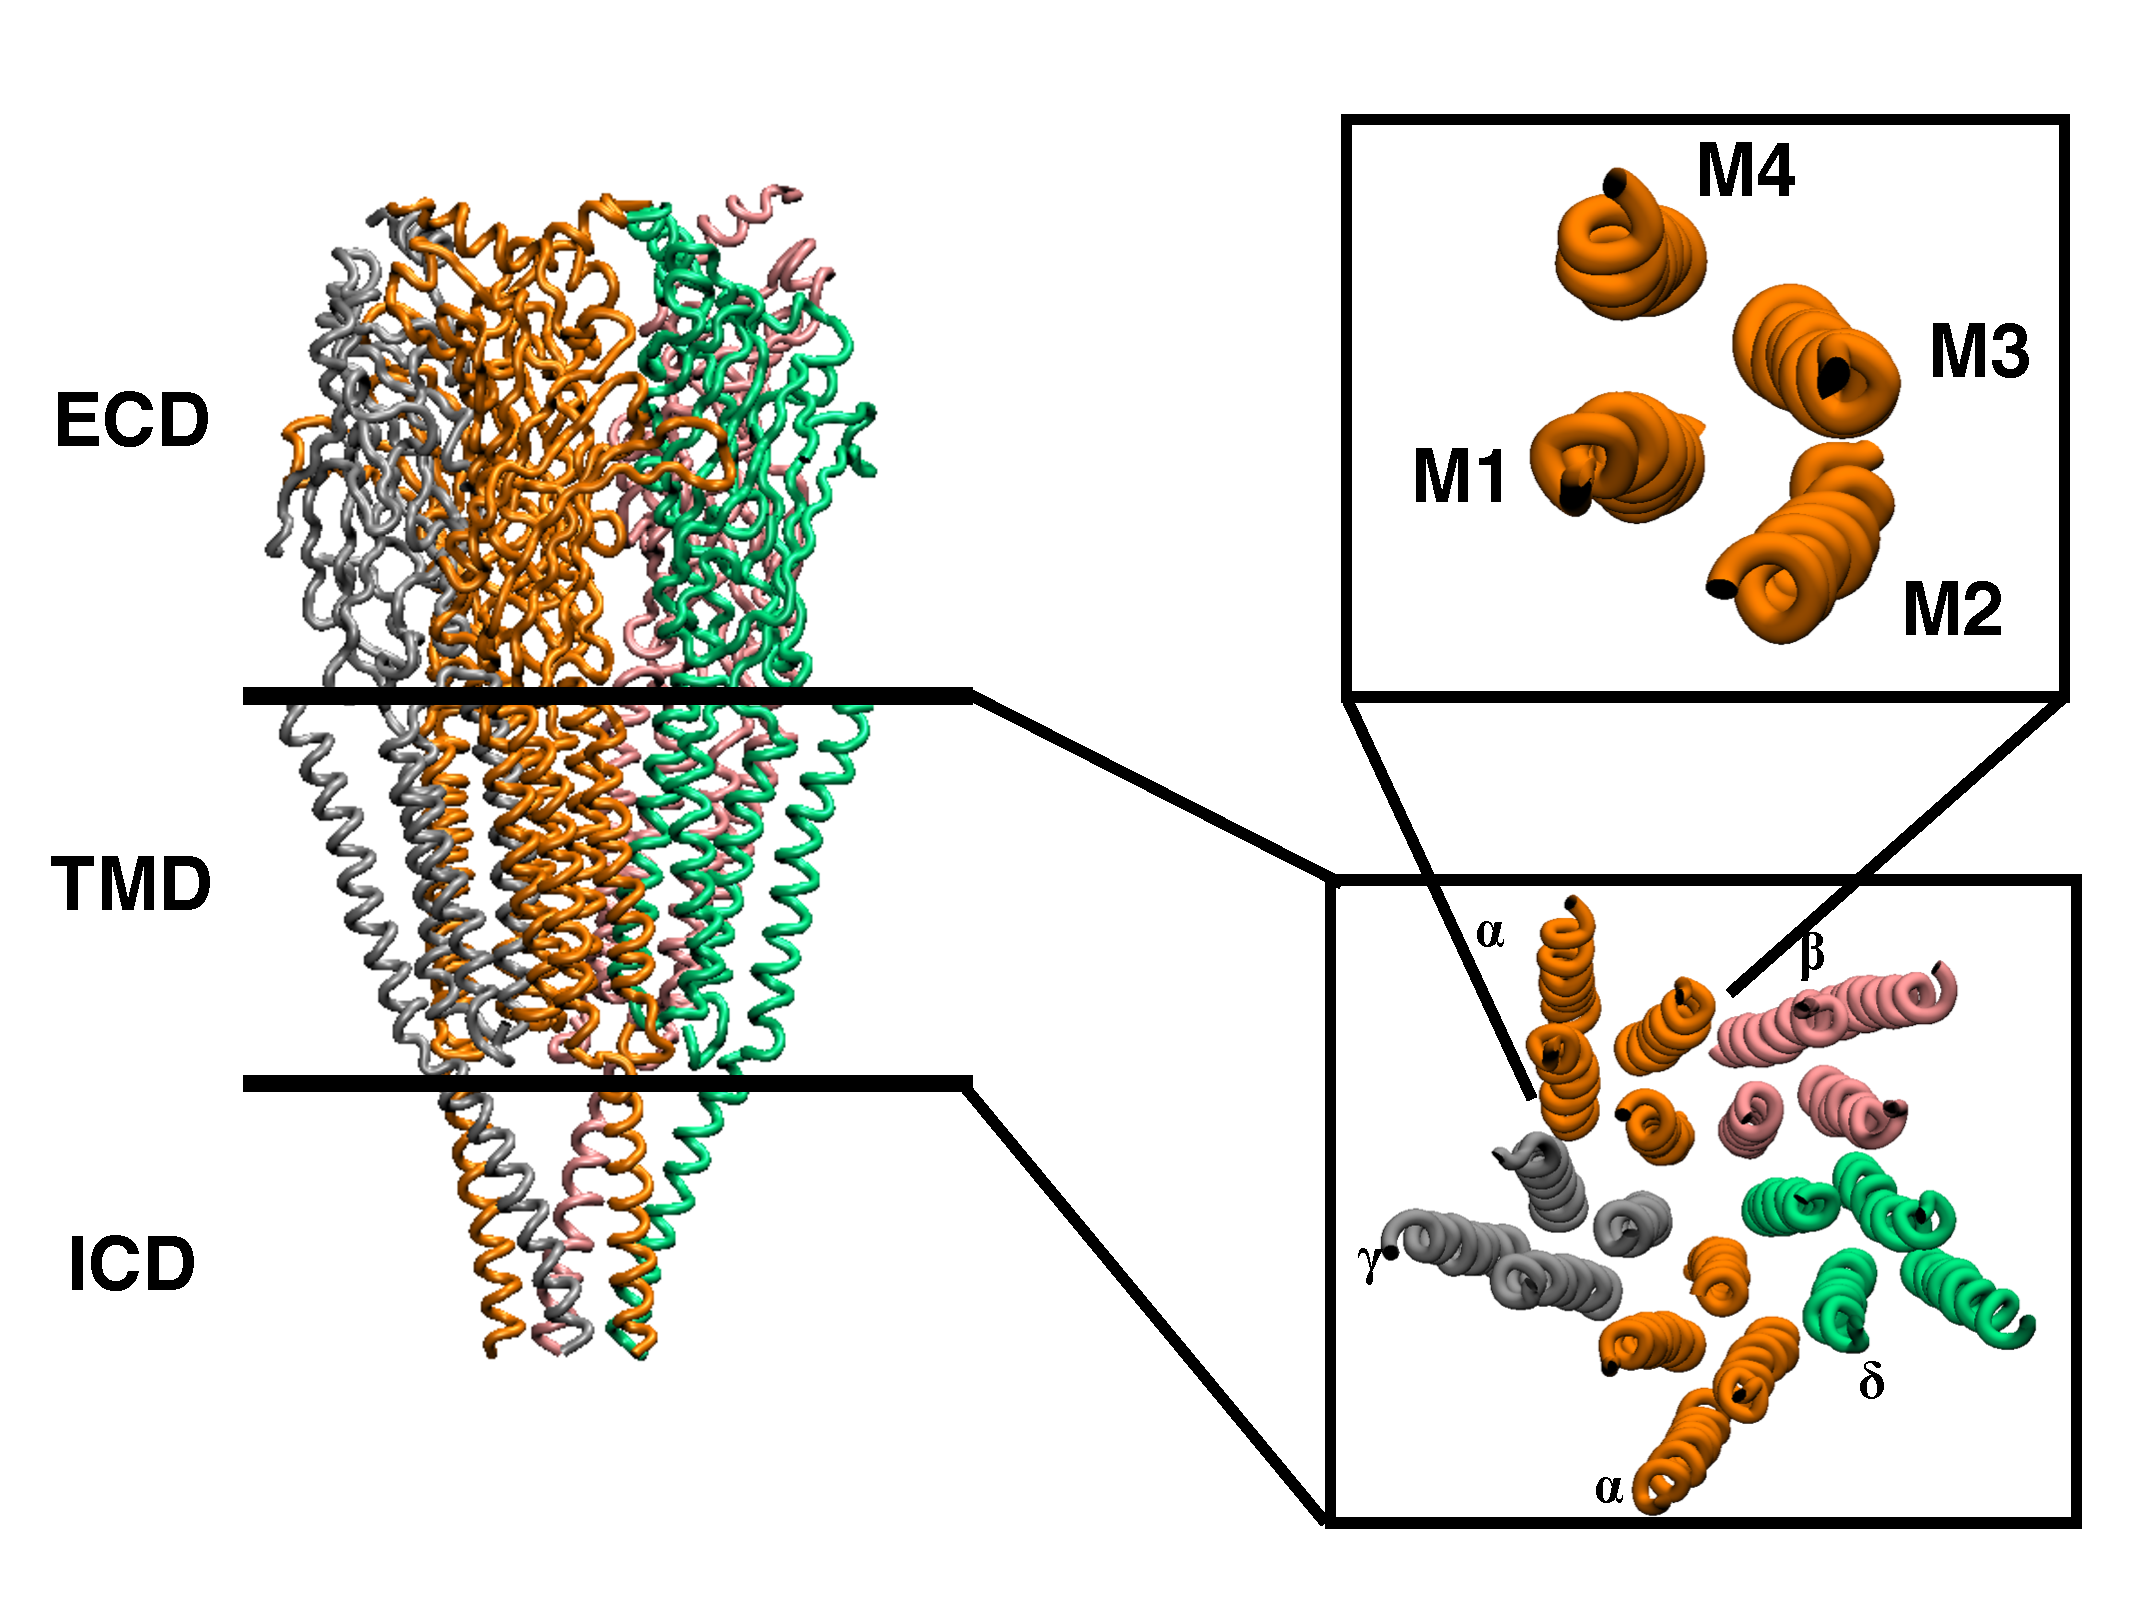
\includegraphics[width=\textwidth,scale=0.5]{domain_nachr.pdf}}
   \caption[nAChR]{ \textbf{nAChR} Above are the domains of nAChR: the Extracellular Domain (ECD), the Transmembrane Domain (TMD), and the Intracellular Domain (ICD). Orange represents $\alpha$ helices. Pink represents $\beta$ helices. Aqua represents $\delta$ helices. Gray represents $\gamma$ helices The subunits are labeled (counter clockwise) $\alpha$ $\gamma$ $\alpha$ $\delta$ $\beta$. Each TMD alpha helix is labeled counter clockwise M1 - M4.
}\label{fig:dom}
\end{figure}
   \newpage

\begin{figure}[H]
   \centerline{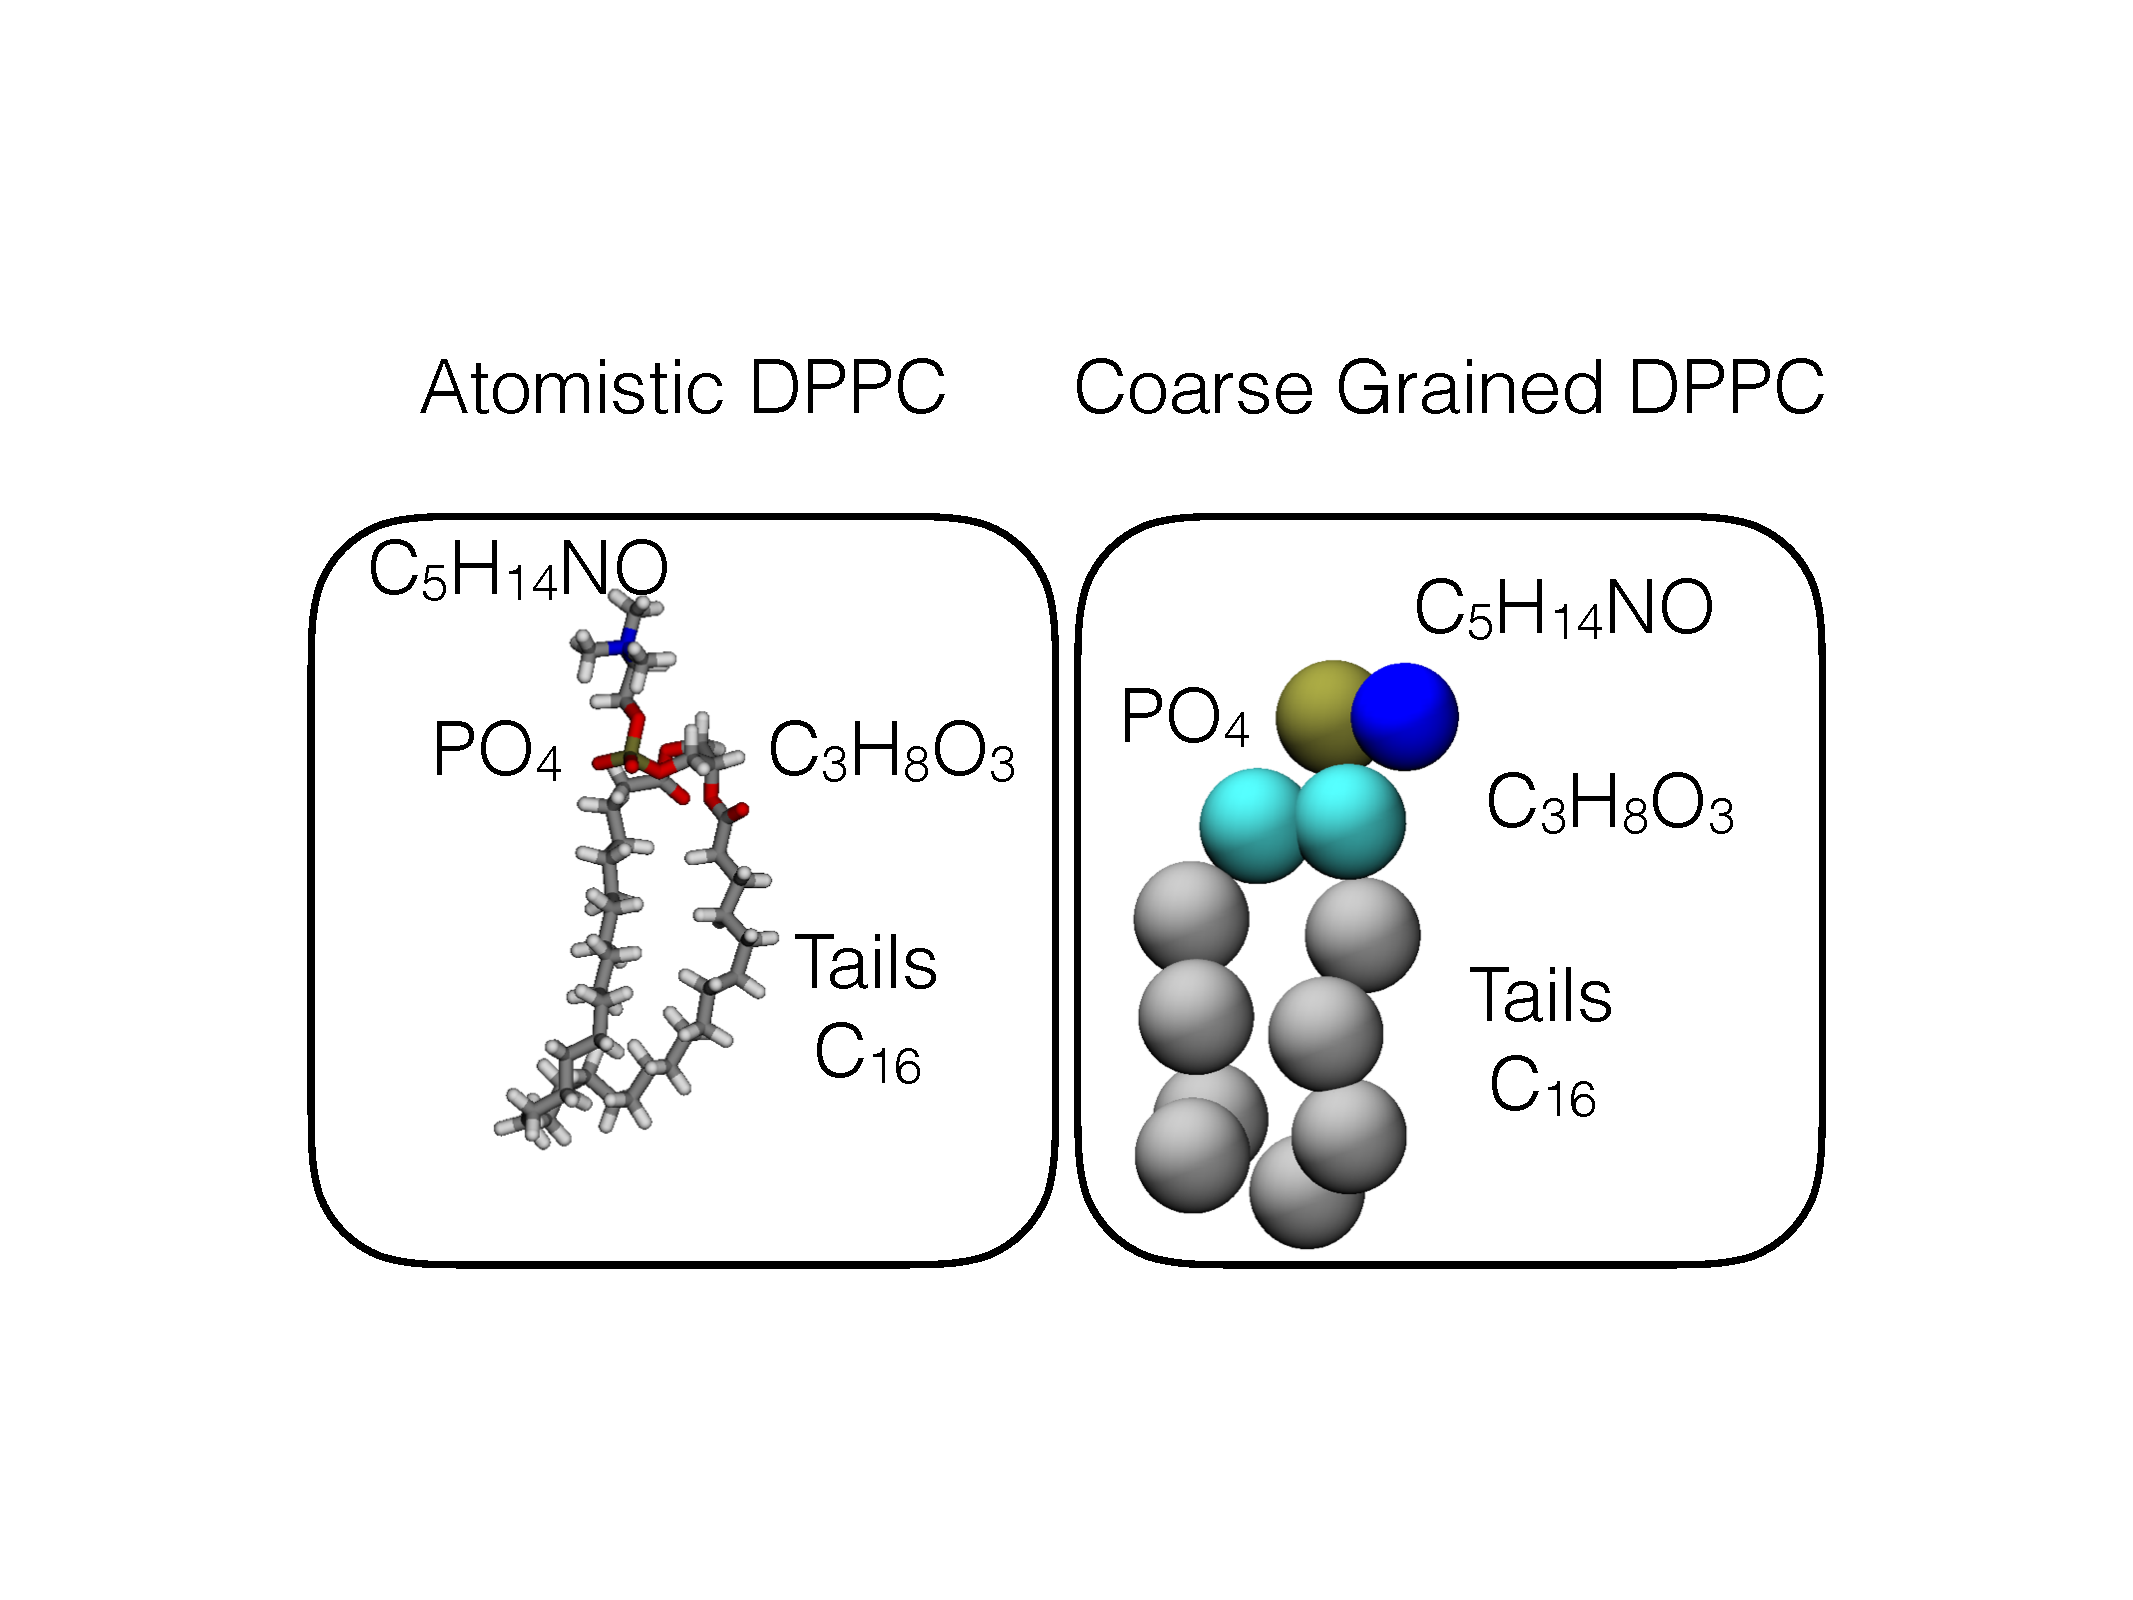
\includegraphics[width=\textwidth,scale=0.5]{CGvAALipids.pdf}}
   \caption[Structural Comparison of All Atomistic and Coarse Grained DPPC]{ \textbf{Structural Comparison of All Atomistic and Coarse Grained DPPC} DPPC viewed as atomistic and coarse grained are compared. The head group PC constructed of phosphocholine (PO$_4$+C$_5$H$_{14}$NO), with a glycerol backbone 2(C$_3$H$_8$O$_3$). Atomistic shows the chemical structure for phosphate, where CG compresses the polyatomic ion to a single bead. This is also seen in C$_5$H$_{14}$NO. In all atomistic, there are 16 carbon atoms a tail. However when viewed in CG, every four atoms are treated as a single bead. 
}\label{fig:AACG}
\end{figure}
   \newpage

\begin{figure}[H]
   \centerline{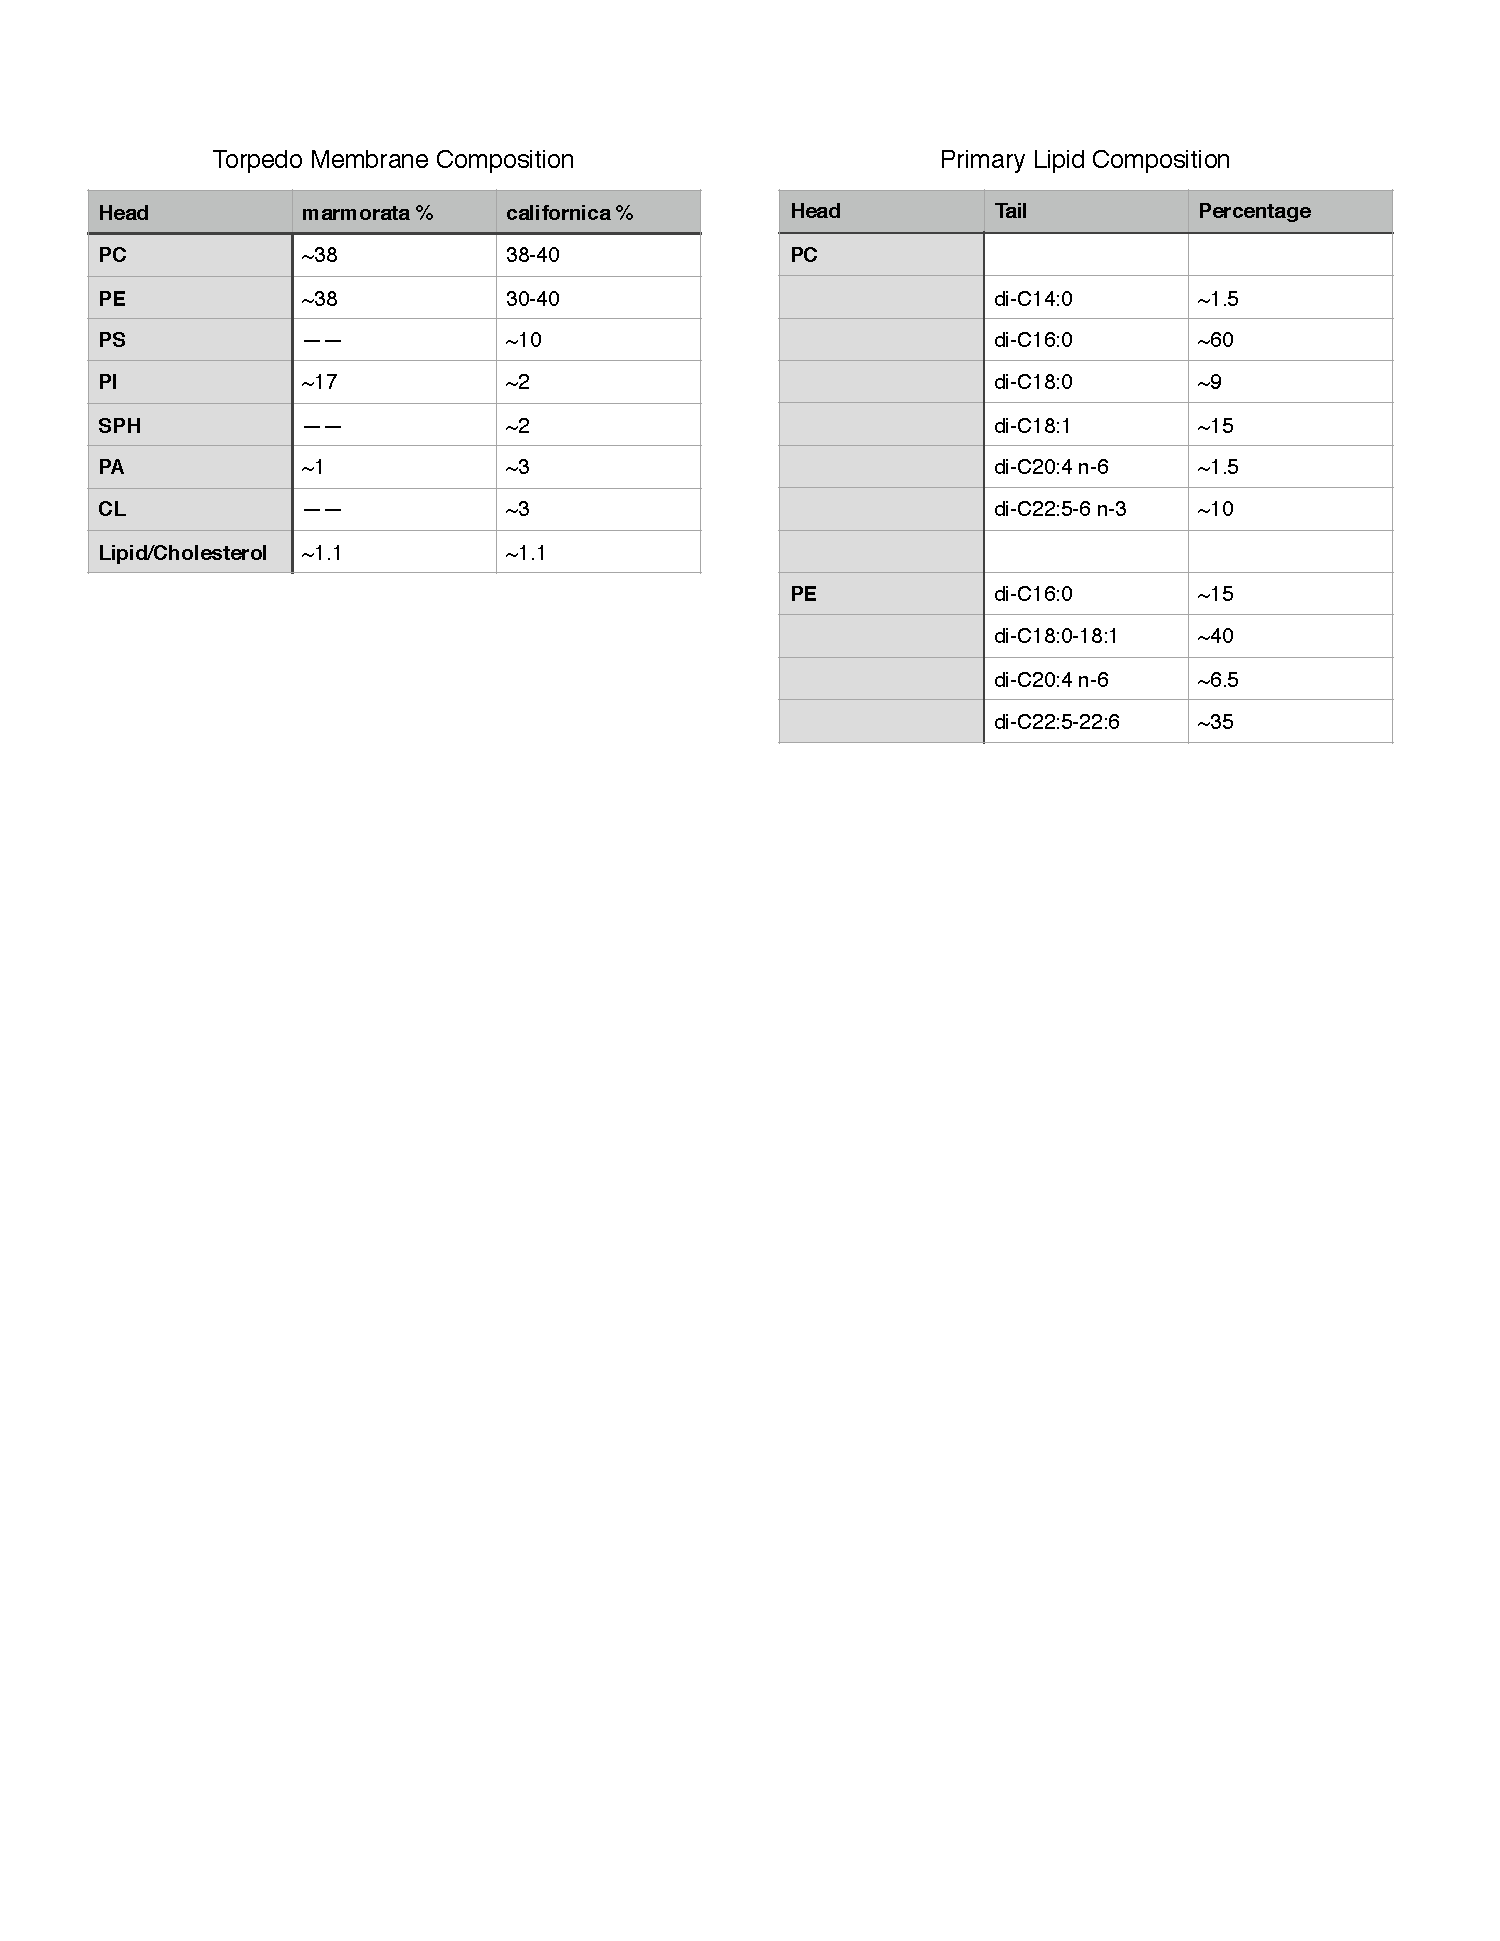
\includegraphics[width=\textwidth,scale=0.75]{Lipid_Bara.pdf}}
   
   \caption[Method of Lipid Choice]{\textbf{Method of Lipid Choice} We wanted lipids that would be observed in the Torpedo electric organ. While nAChR activates with cholesterol and lipids with PA head groups, PA did not make up a significant amount of the membrane based on Barantes work. Where PC = Phosphocholine, PE = Phosphatidylethanolamine, PS = Phosphatidylserine, PI = Phosphatidylinositol, PG = Phosphatidylglycerol, SPH = sphingomyelin, PA = Phosphatidic acid, and CL = Diphosphatidylglycerol \cite{barrantesthe1989}.
}\label{fig:lchart1}

\end{figure}
\newpage
\begin{figure}[H]
   \centerline{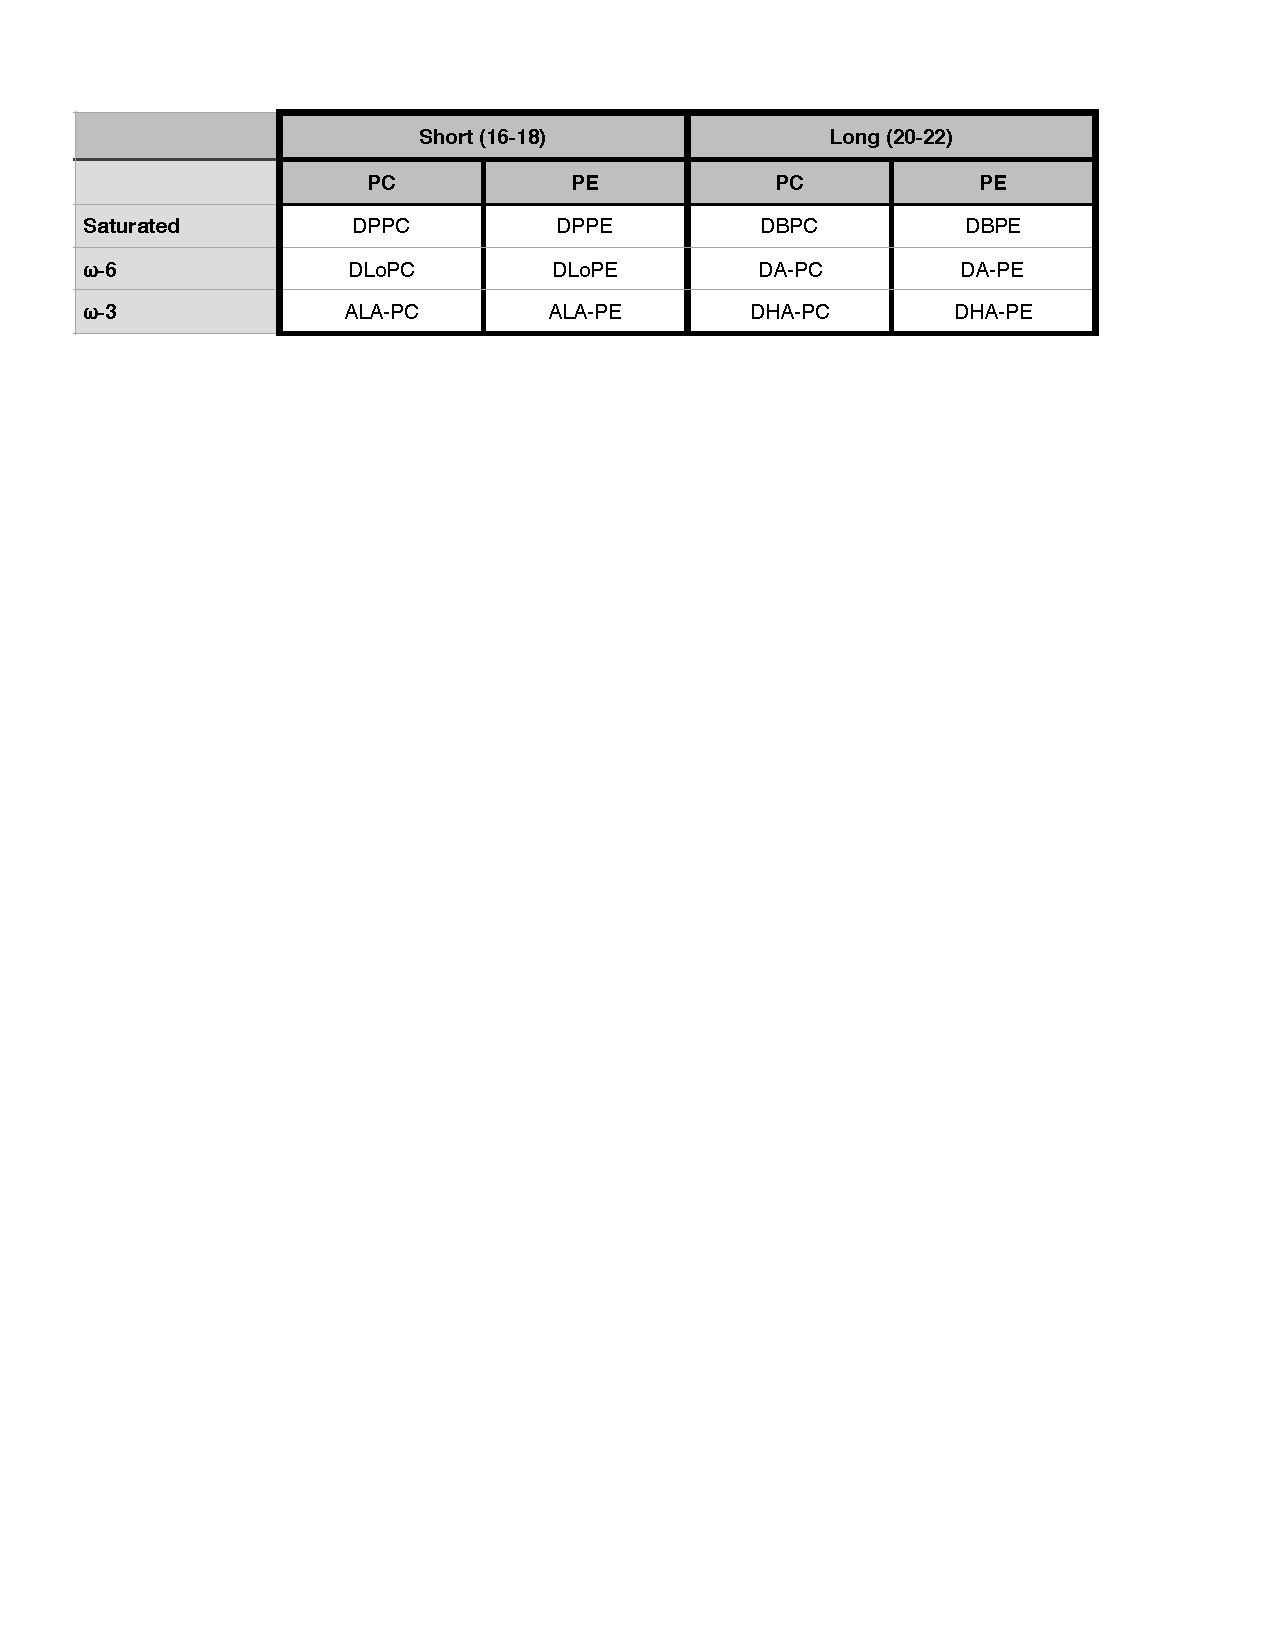
\includegraphics[width=\textwidth,scale=1]{Lipid_Table.pdf}}
   
   \caption[Lipid Tail Length and Saturation]{\textbf{Lipid Tail Length and Saturation} Above organizes lipids used in our simualtions by their tail lengths and saturation.
   }\label{fig:lchart2}

\end{figure}
   \newpage

\begin{figure}[H]
   \centerline{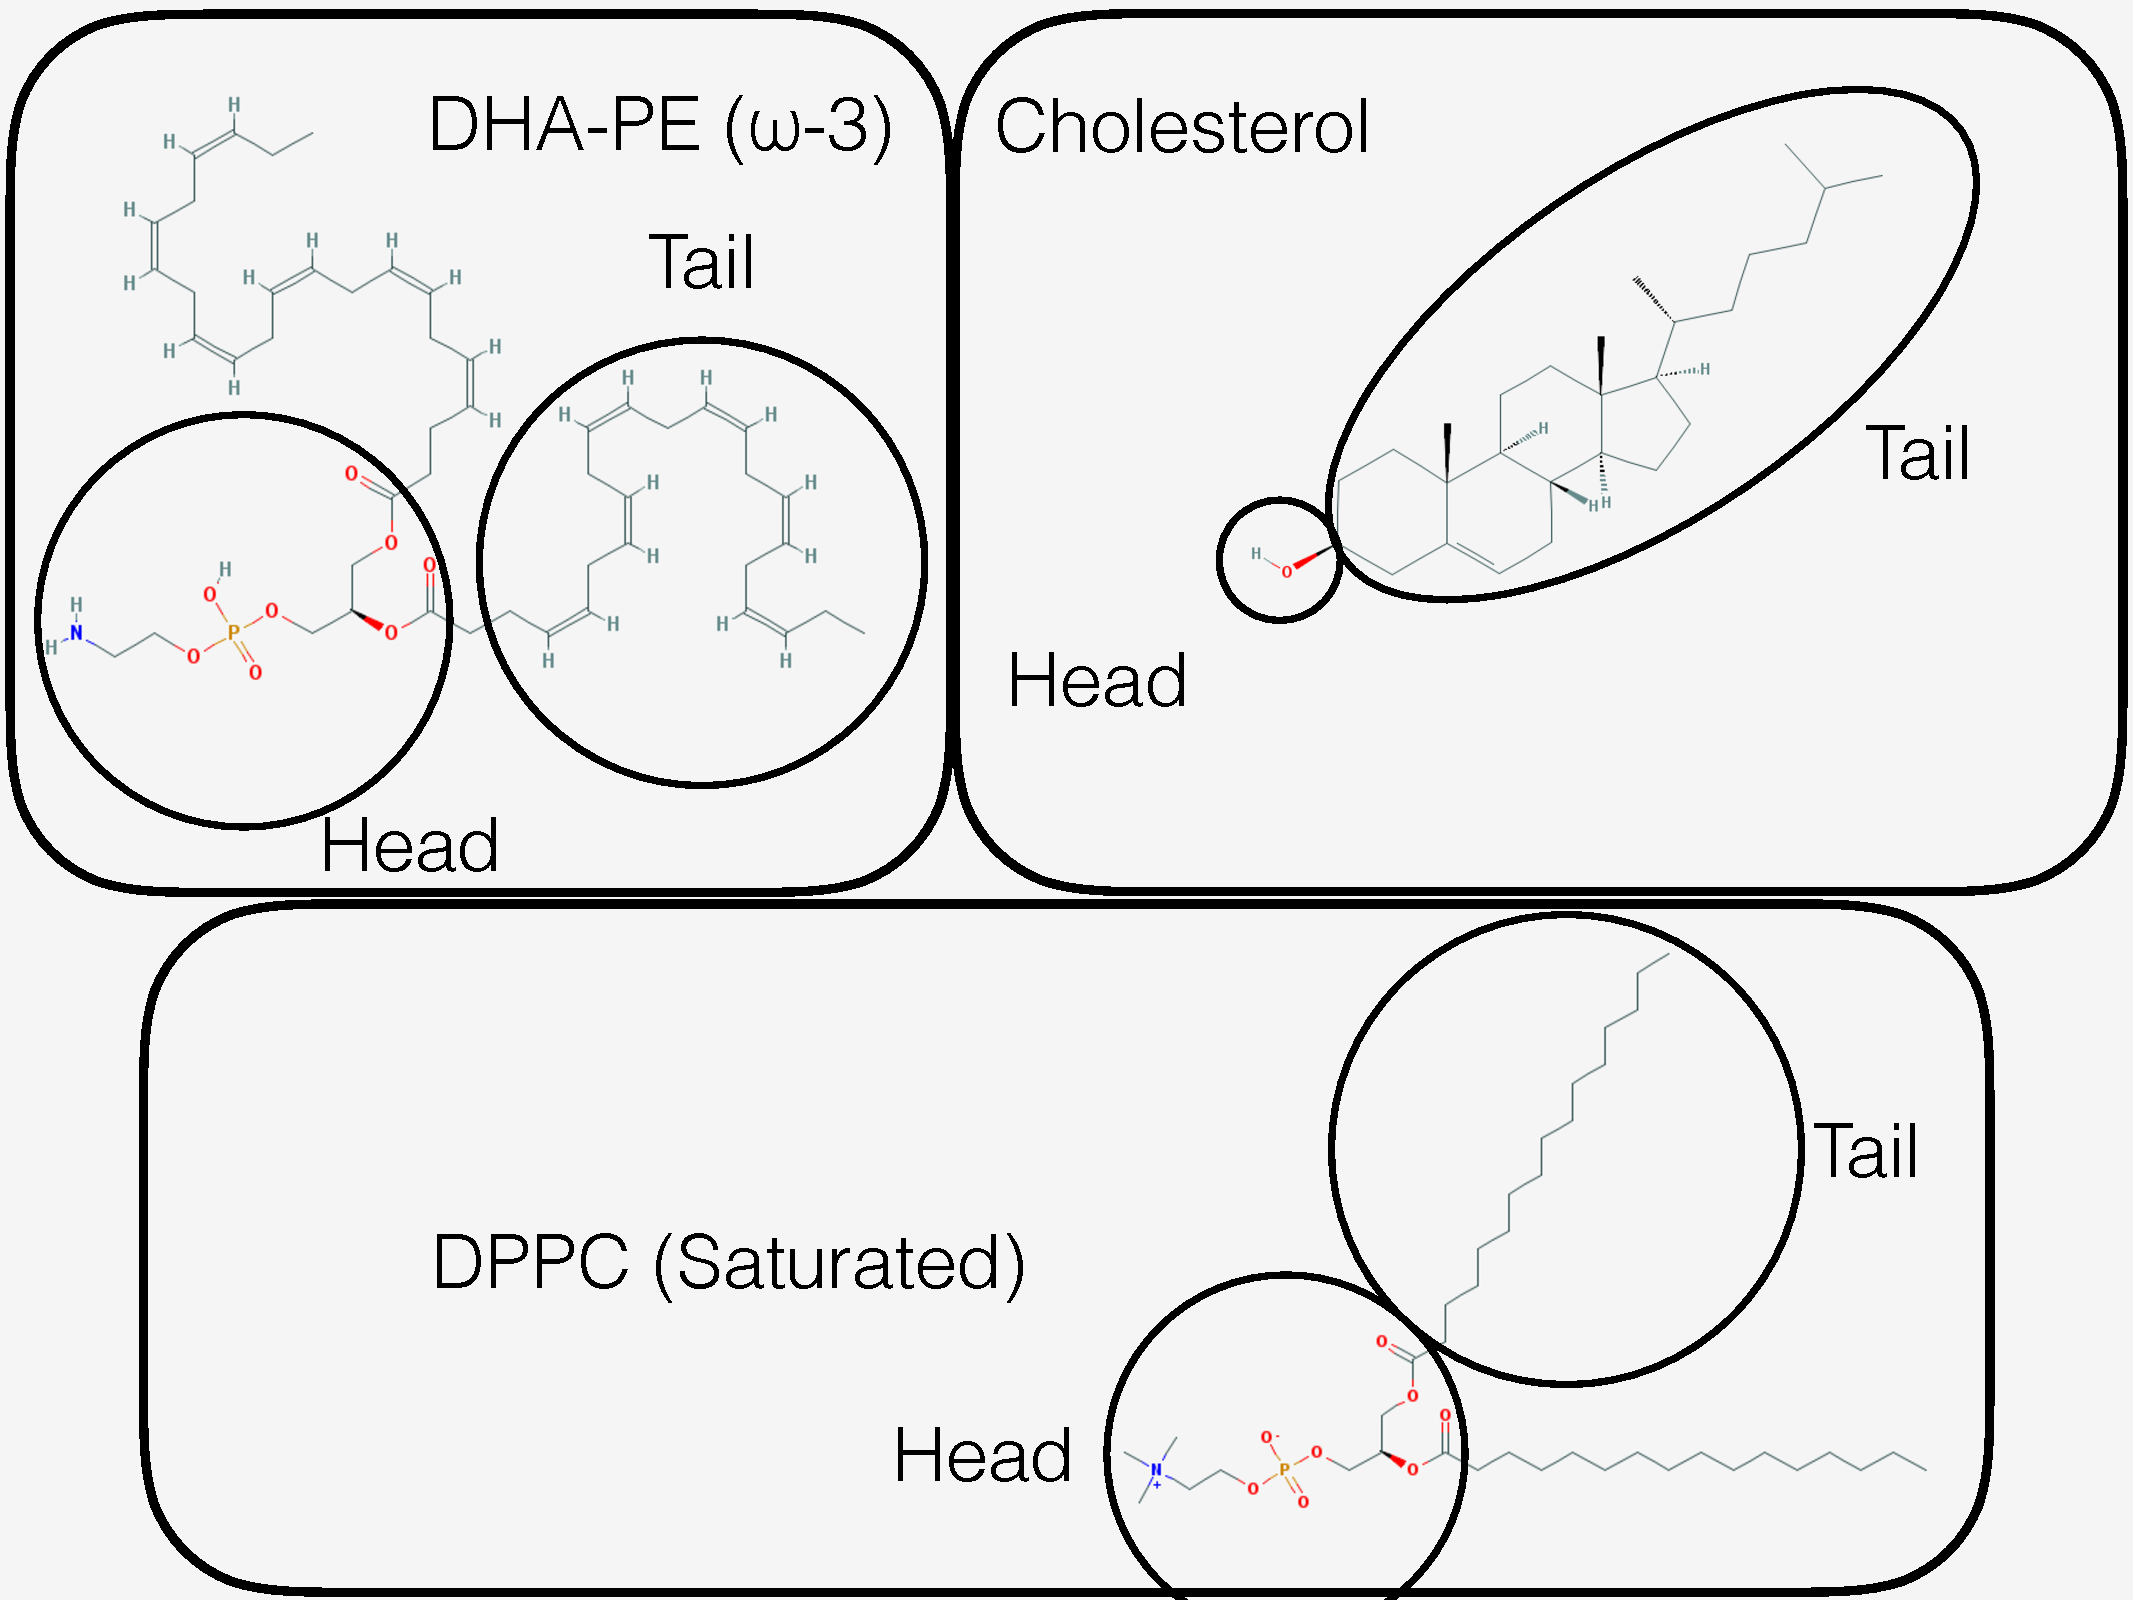
\includegraphics[width=\textwidth,scale=0.55]{Lipid_struct.pdf}}
   \caption[Lipid Structure]{\textbf{Lipid Structure} We present three lipids DHA-PE, cholesterol, and DPPC. DHA-PE, cholesterol, and DPPC head groups are phosphatidylethanolamine with a glycerol backbone, hydroxide, and phosphocholine with a glycerol backbone. The head and tail groups of each molecule is circled. \cites{cholesterol}{dppc}{pe(22:6/22:6)}.
}\label{fig:chol}

\end{figure}
   \newpage

\begin{figure}[H]

   \centerline{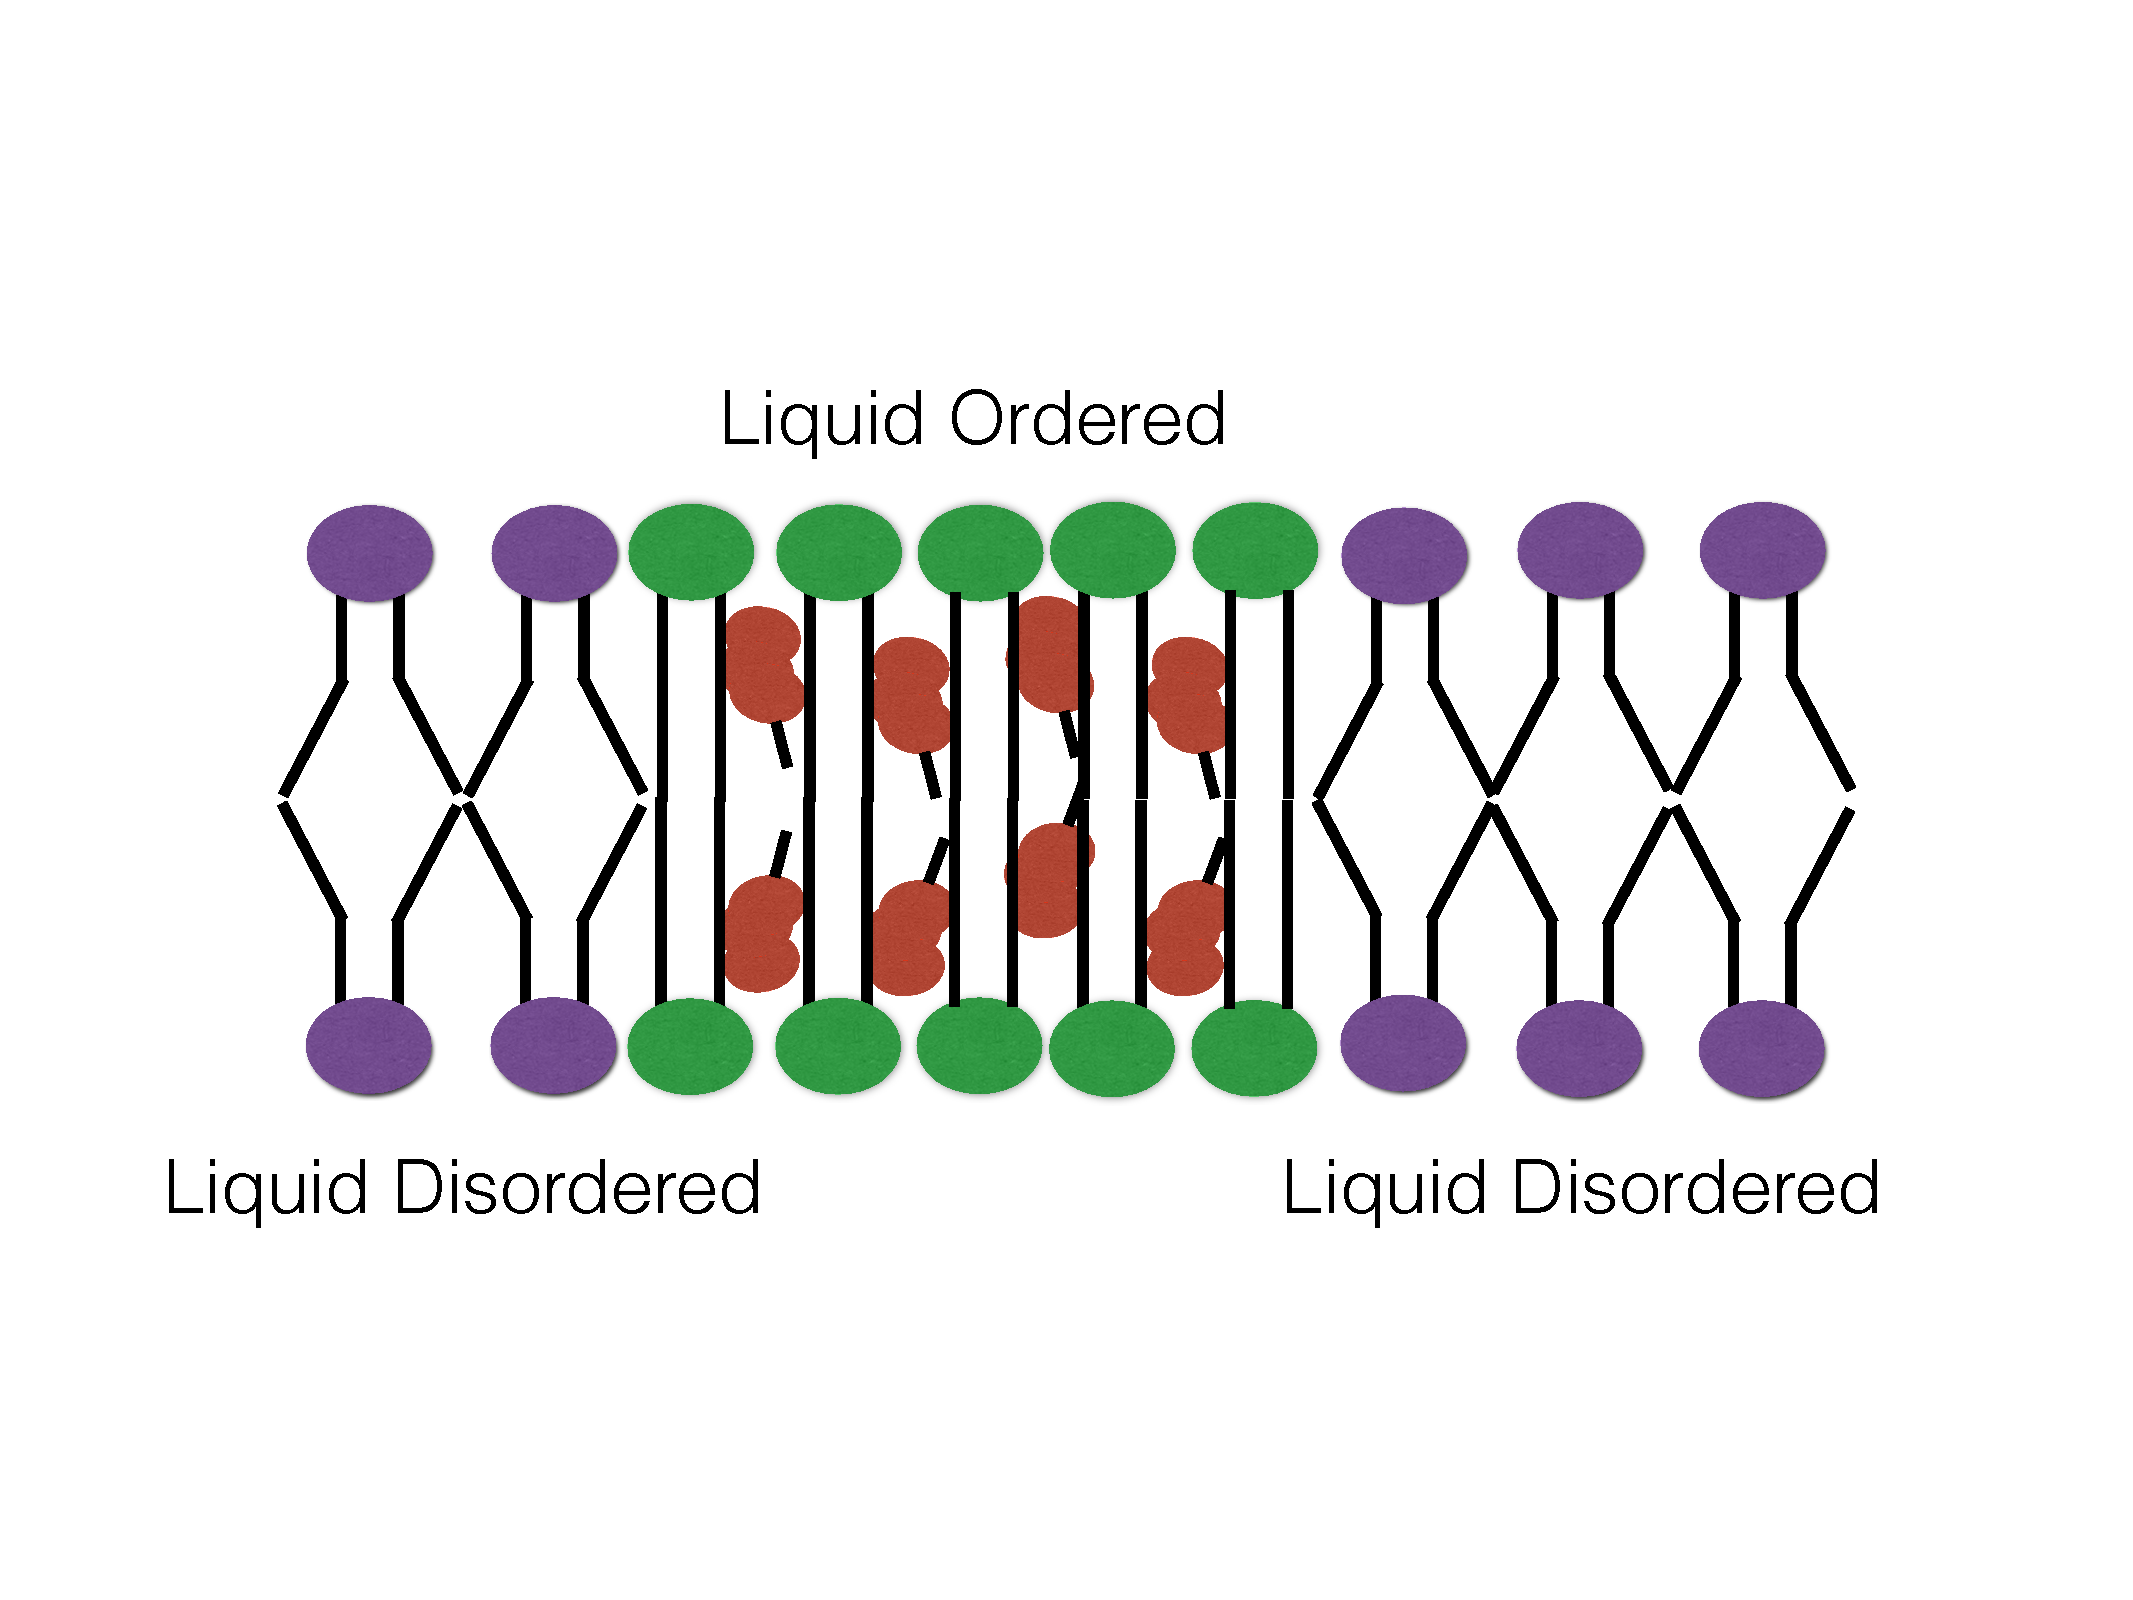
\includegraphics[width=\textwidth,scale=0.5]{bilayCartoon.pdf}}
   \caption[Raft Formation]{\textbf{Raft Formation} Above is an example of lipid raft formation. Cholesterol (red) and a generic saturated lipid (green) aggregate together, de-mixing from the generic polyunsaturated lipid (purple)and forming two phases: liquid ordered and disordered.}\label{fig:clips}

\end{figure}
\newpage

\begin{figure}[H]

   \centerline{\includegraphics[width=\textwidth,scale=0.5]{Lipid_Img.pdf}}
   \caption[Membranes Containing 15\% Cholesterol with an Embedded Protein]{\textbf{Membranes Containing 15\% Cholesterol with an Embedded Protein} Membranes containing 15\% cholesterol and 42.5\% DPPC and 42.5\% of one secondary lipid. Images are organized based on tail length and saturation. Lipids with longer tails appear to have more defined domains. nAChR partitions into the liquid disordered domain.}\label{fig:plips}

\end{figure}
\newpage

\begin{figure}[H]

   \centerline{\includegraphics[width=\textwidth,scale=0.5]{memb_Lipid}}
   \caption[Membranes Containing 15\% Cholesterol]{\textbf{Membranes Containing 15\% cholesterol} Membranes containing 15\% cholesterol and 42.5\% DPPC and 42.5\% of one secondary lipid. Images are organized based on tail length and saturation. Lipids with longer tails appear to have more defined domains.}\label{fig:mlips}

\end{figure}
\newpage

\begin{figure}[H]

   \centerline{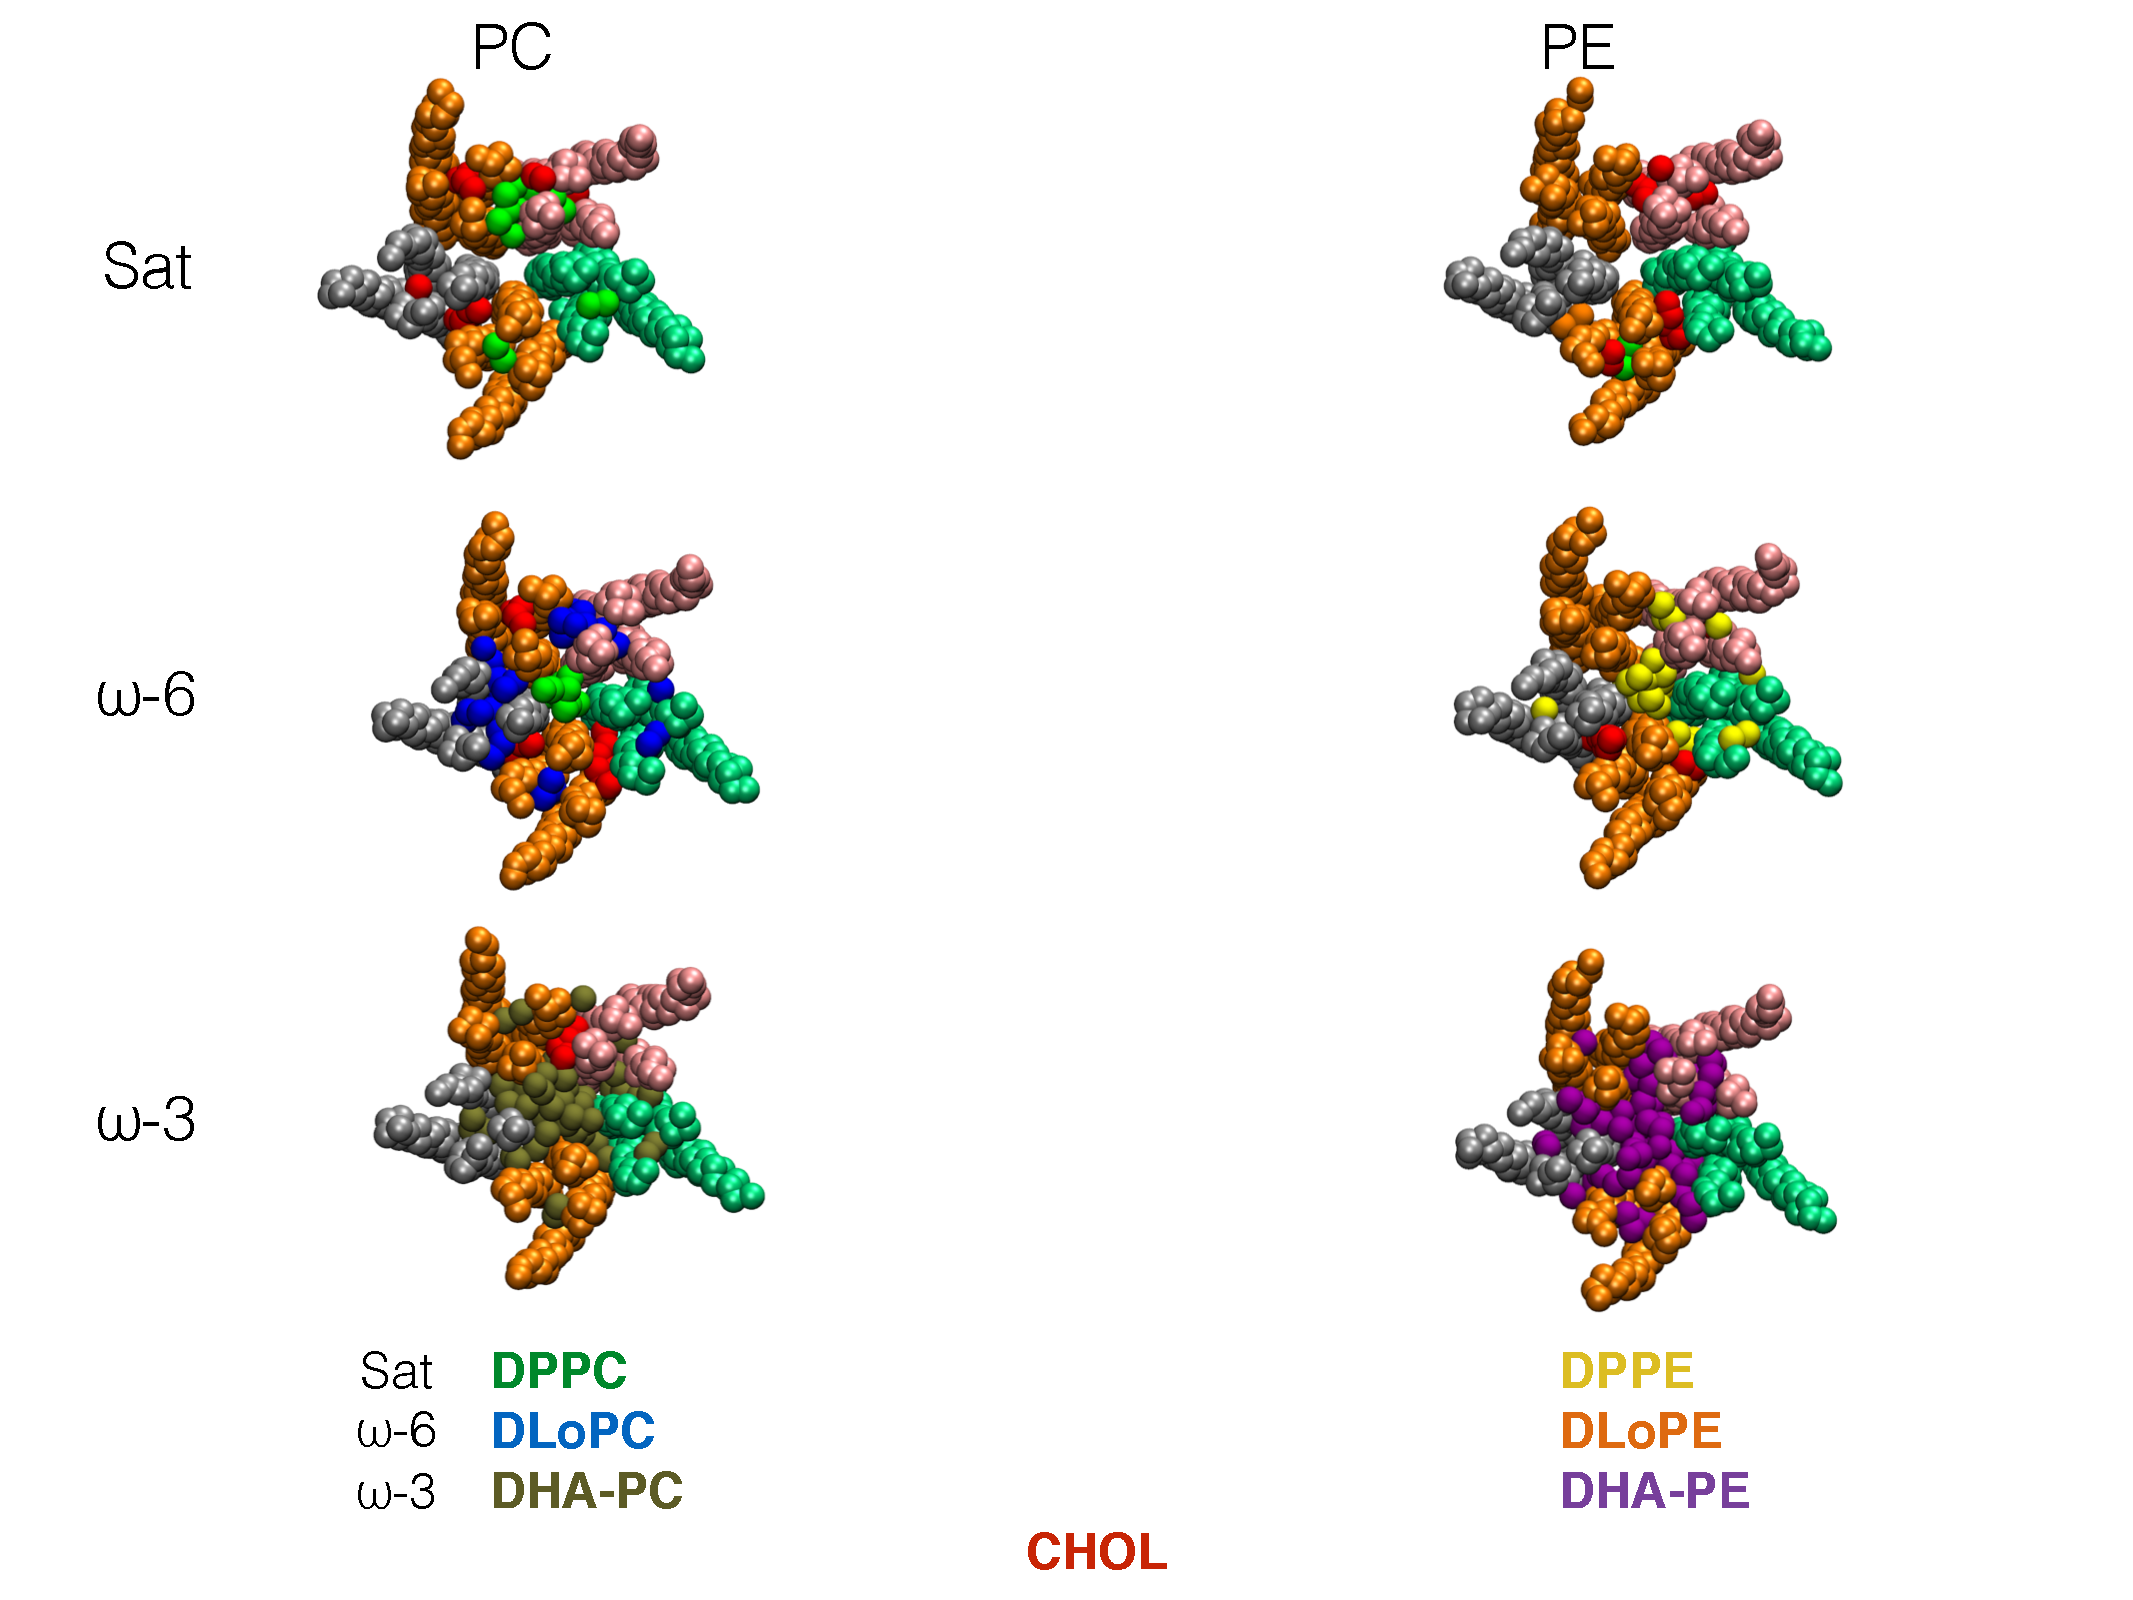
\includegraphics[width=\textwidth,scale=0.5]{Embeded_Lip}}
   \caption[Simulations Containing 15\% Cholesterol: Embedded Lipids]{\textbf{Simulations Containing 15\% Cholesterol: Embedded Lipids} Shown are lipids embedded in protein. All membranes containing 15\% cholesterol and 42.5\% DPPC and 42.5\% of one secondary lipid. Images are organized based on tail length and saturation.}\label{fig:elips}

\end{figure}
\newpage

\begin{figure}[H]
   \centerline{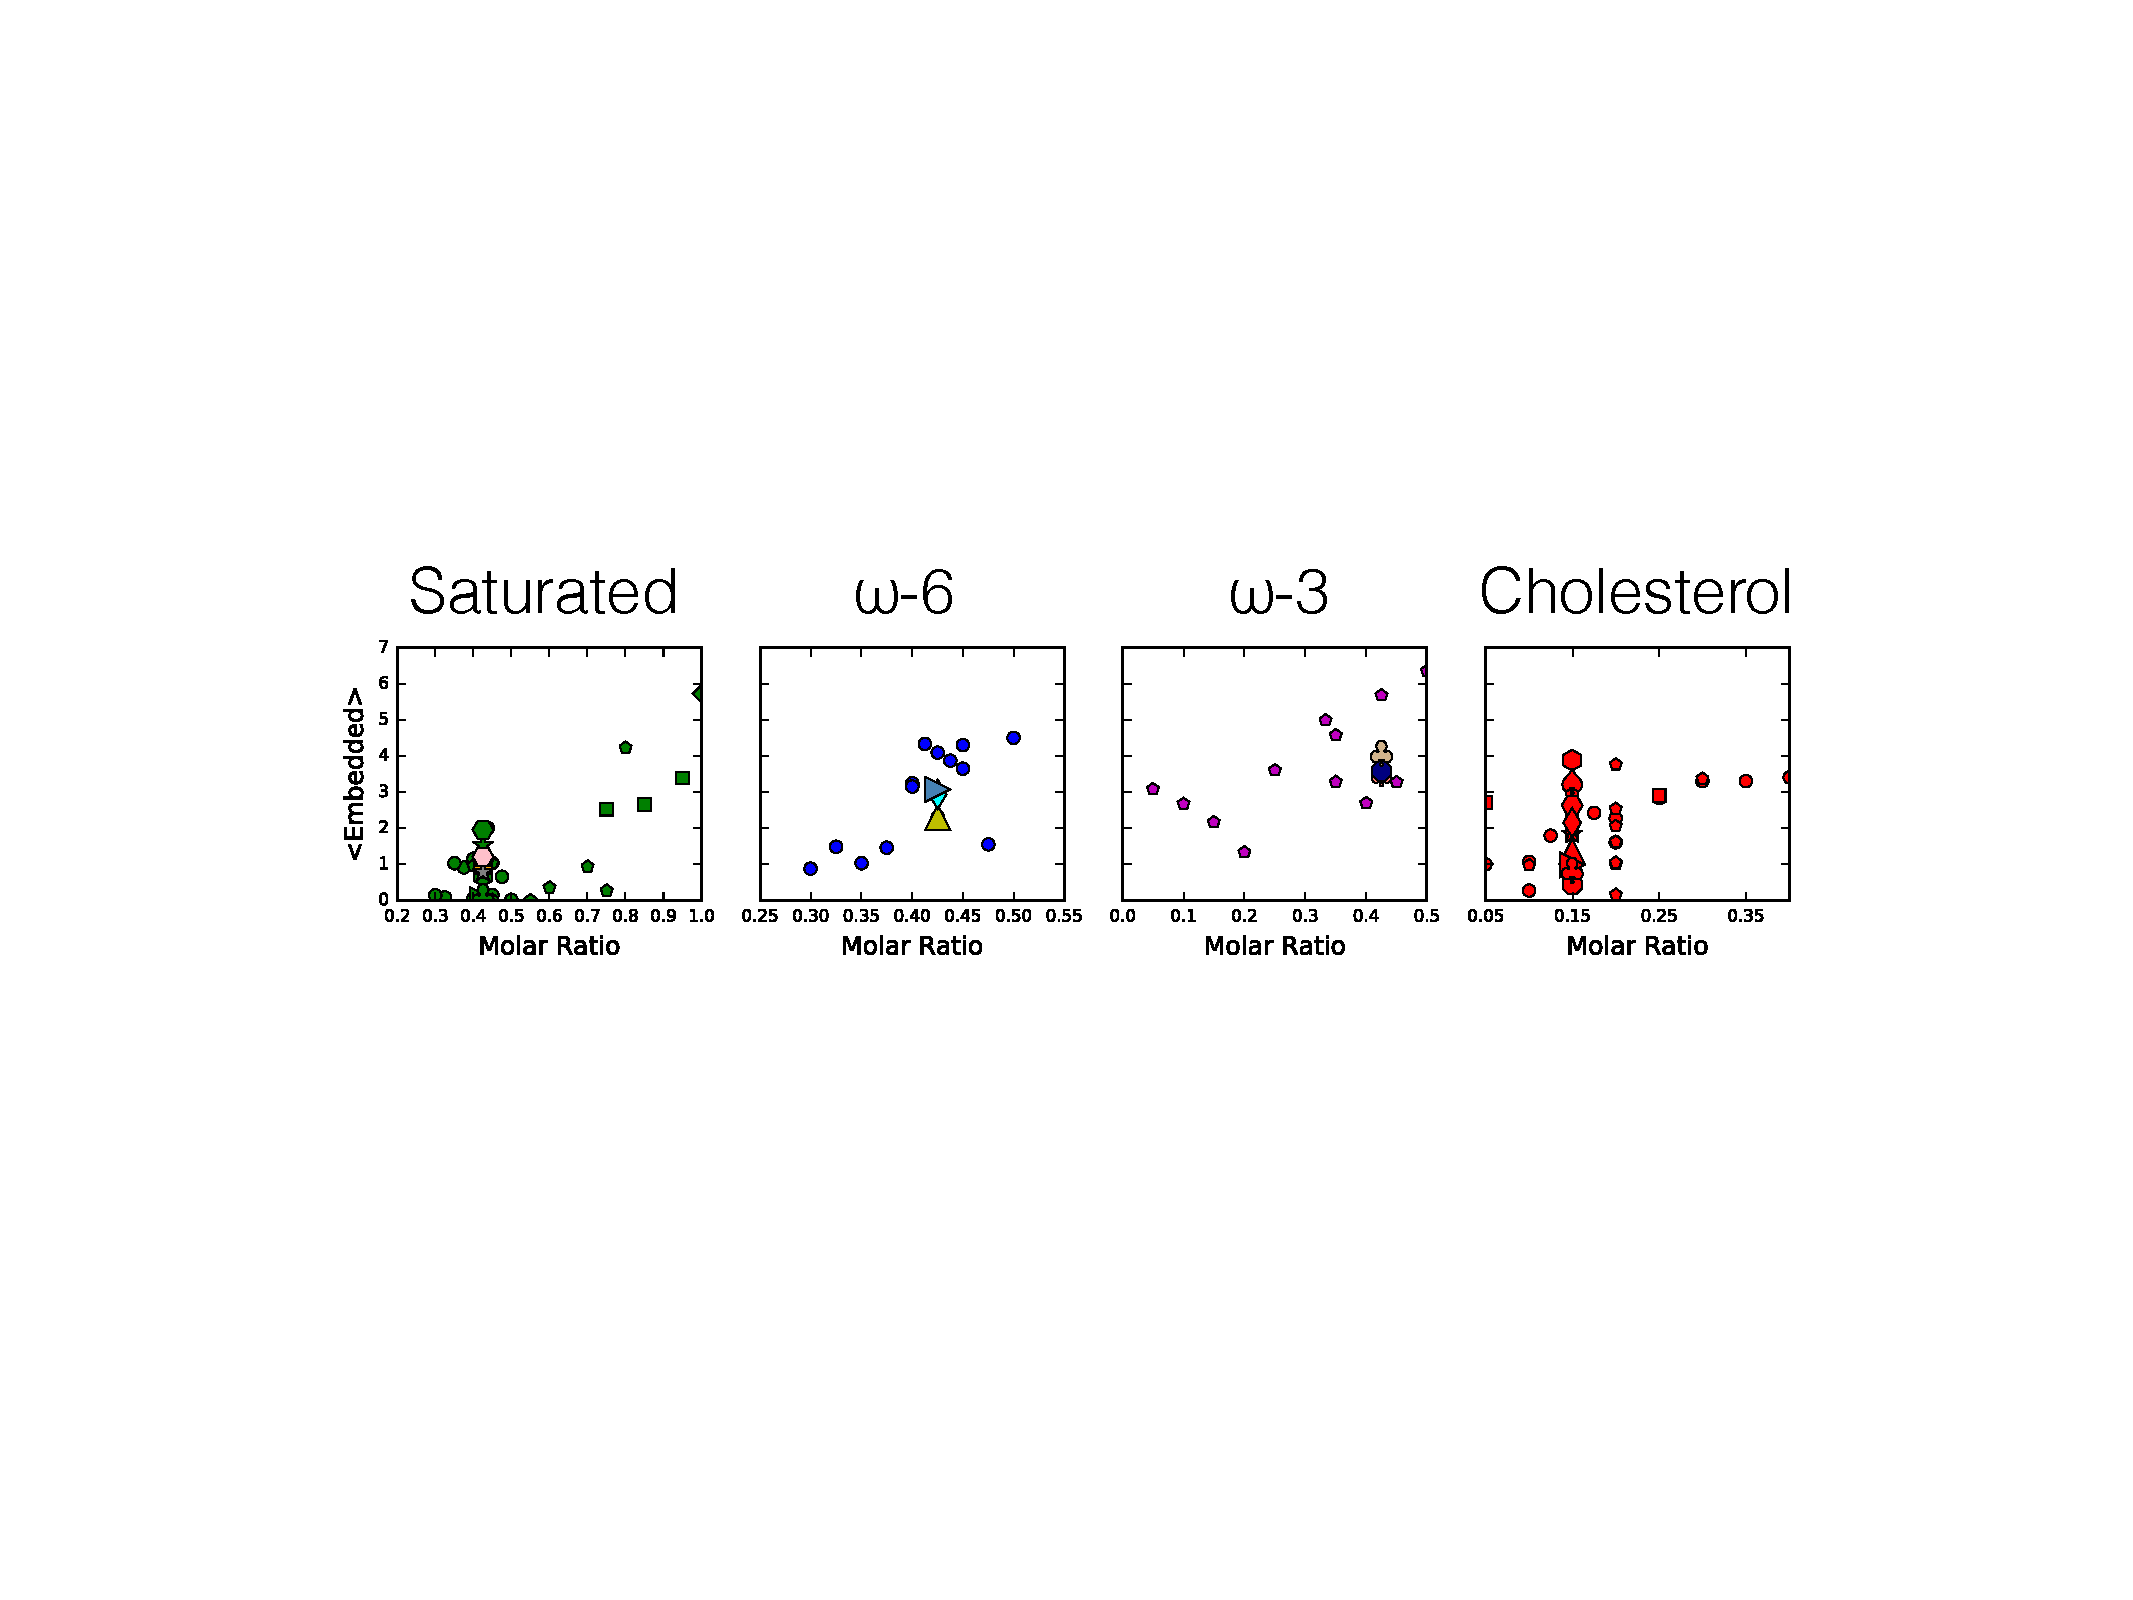
\includegraphics[width=\textwidth,scale=0.5]{Embeded_plot.pdf}}
   \centerline{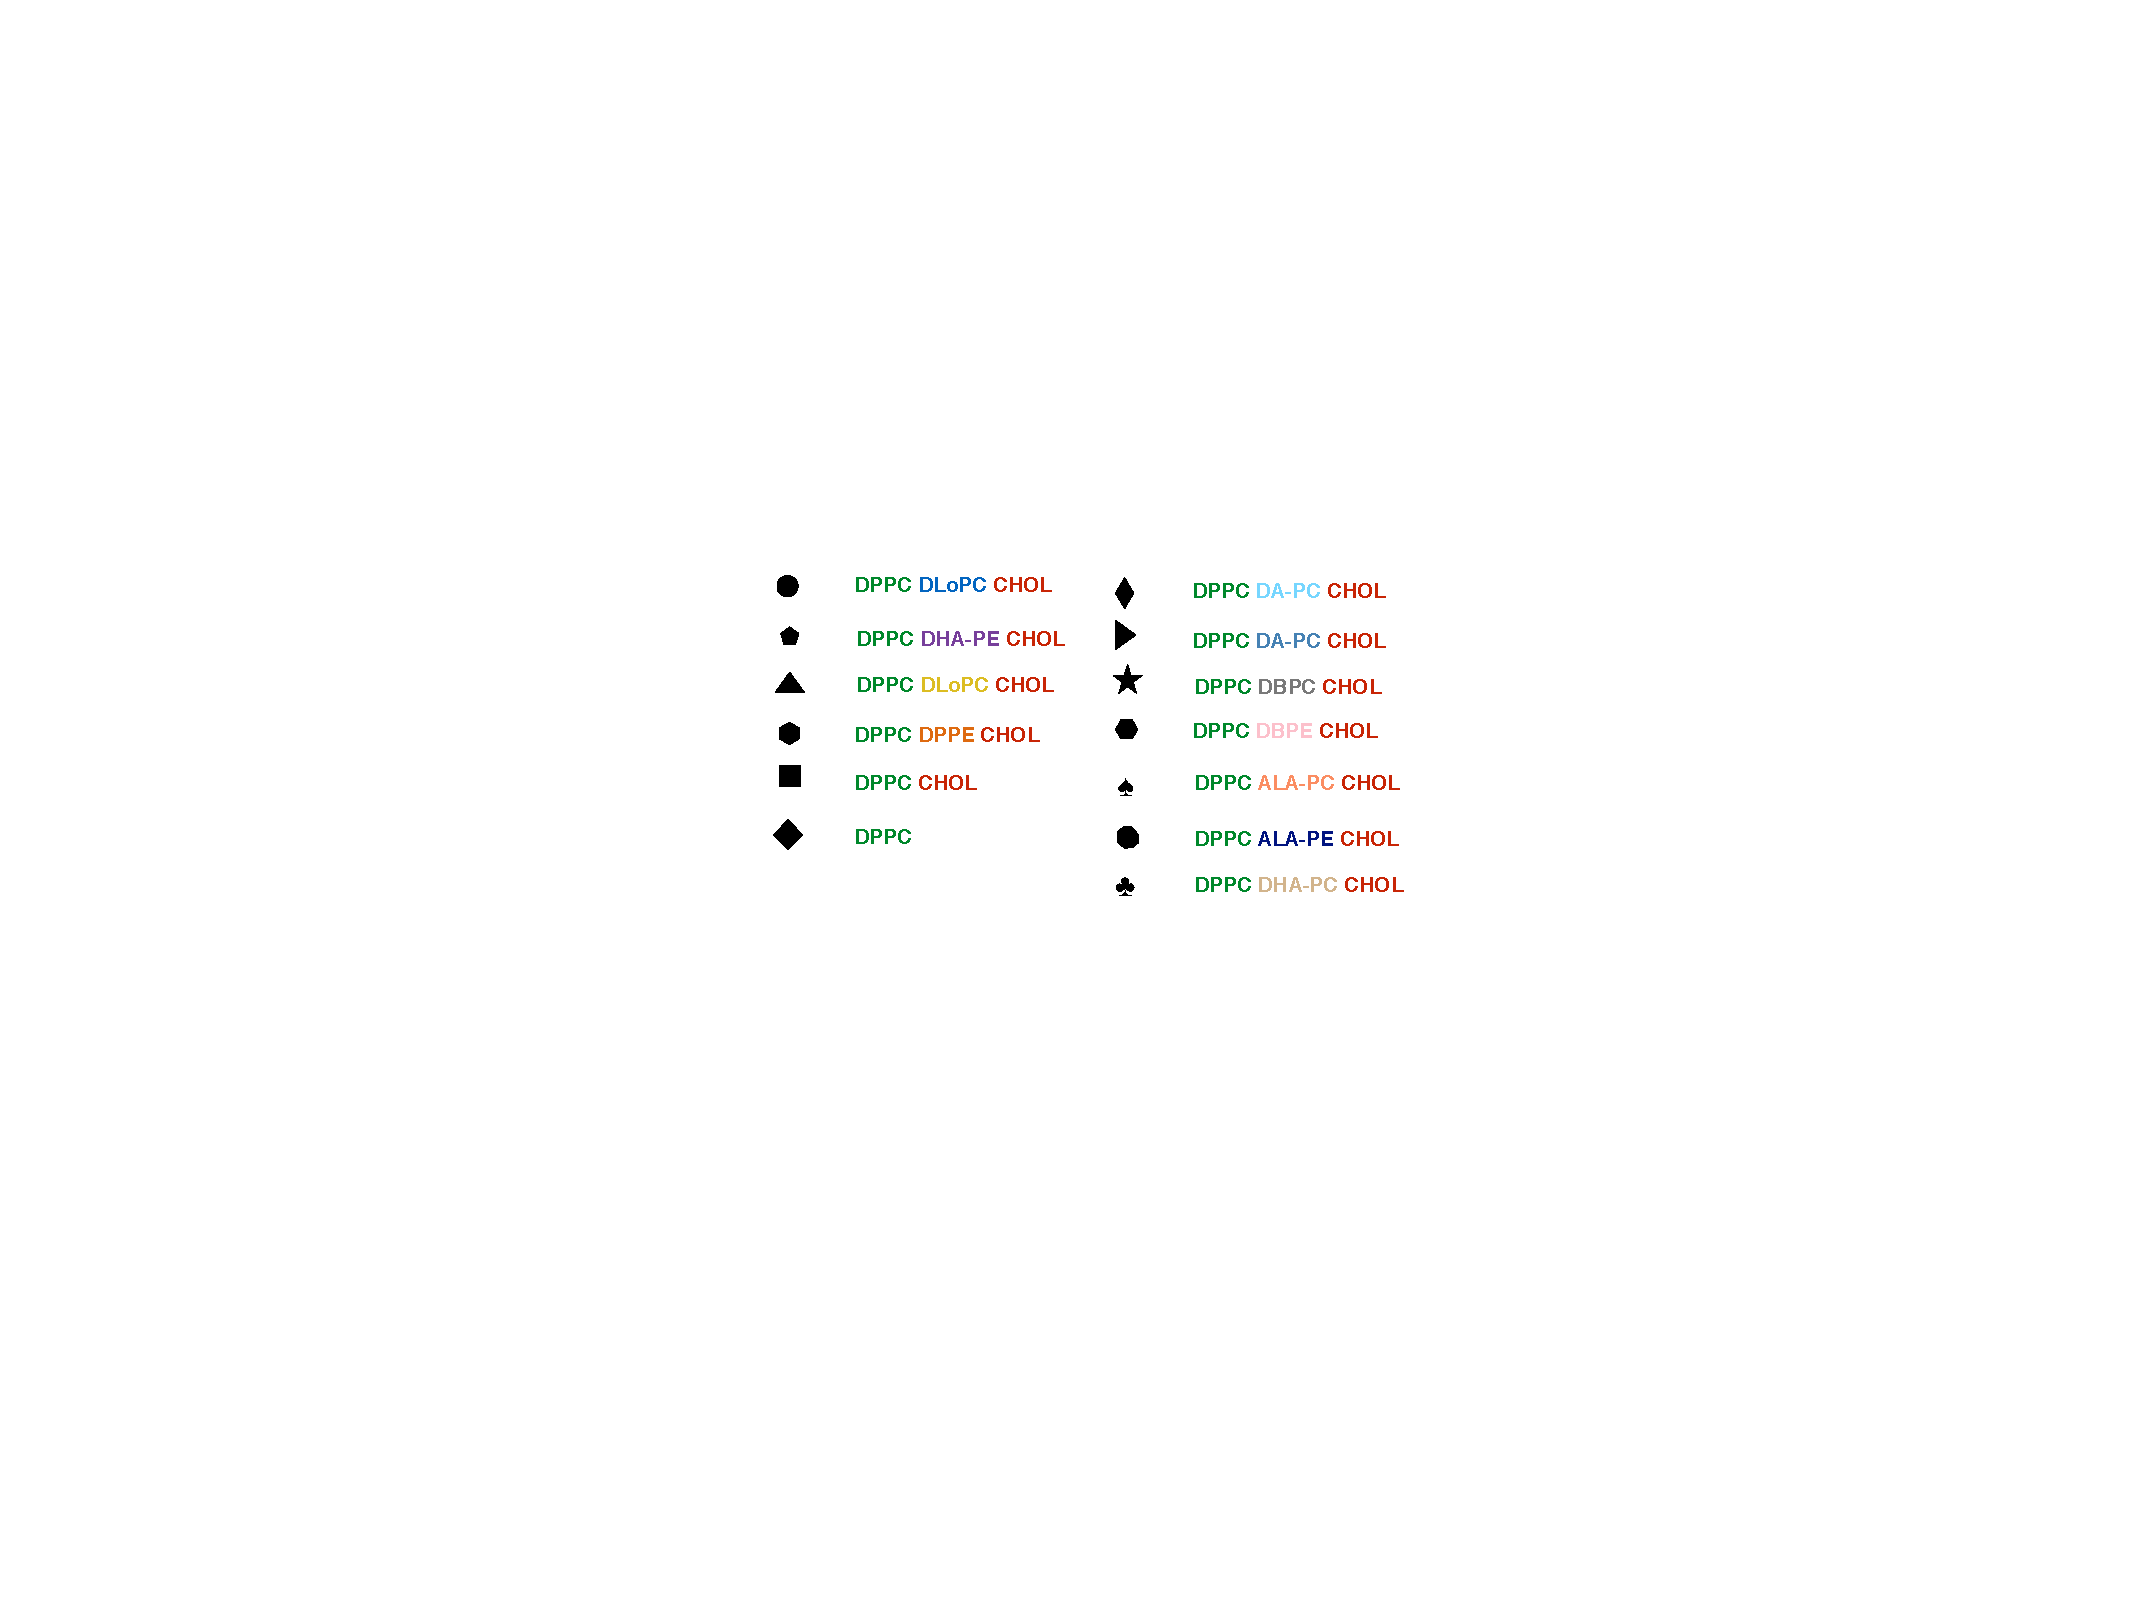
\includegraphics[scale=0.45]{Legend.pdf}}
   \caption[Quantitative Analysis of Non-Annular Deep Binding of Lipids in nAChR]{\textbf{Quantitative Analysis of Non-Annular Deep Binding of Lipids in nAChR} Non-Annular deep binding of lipids in nAChR is shown to occur in all systems. However, polyunsaturated lipids and cholesterol are more likely to embed than saturated lipids. Each plot represents one type of lipid we observed to embed. Embedding appears to be a function of the concentration of lipids and species of lipids. Each point is the average count of a given lipid species over the final 1.5 $\mu$s}\label{fig:emb}

 \end{figure}
\newpage


\begin{figure}[H]
   \centerline{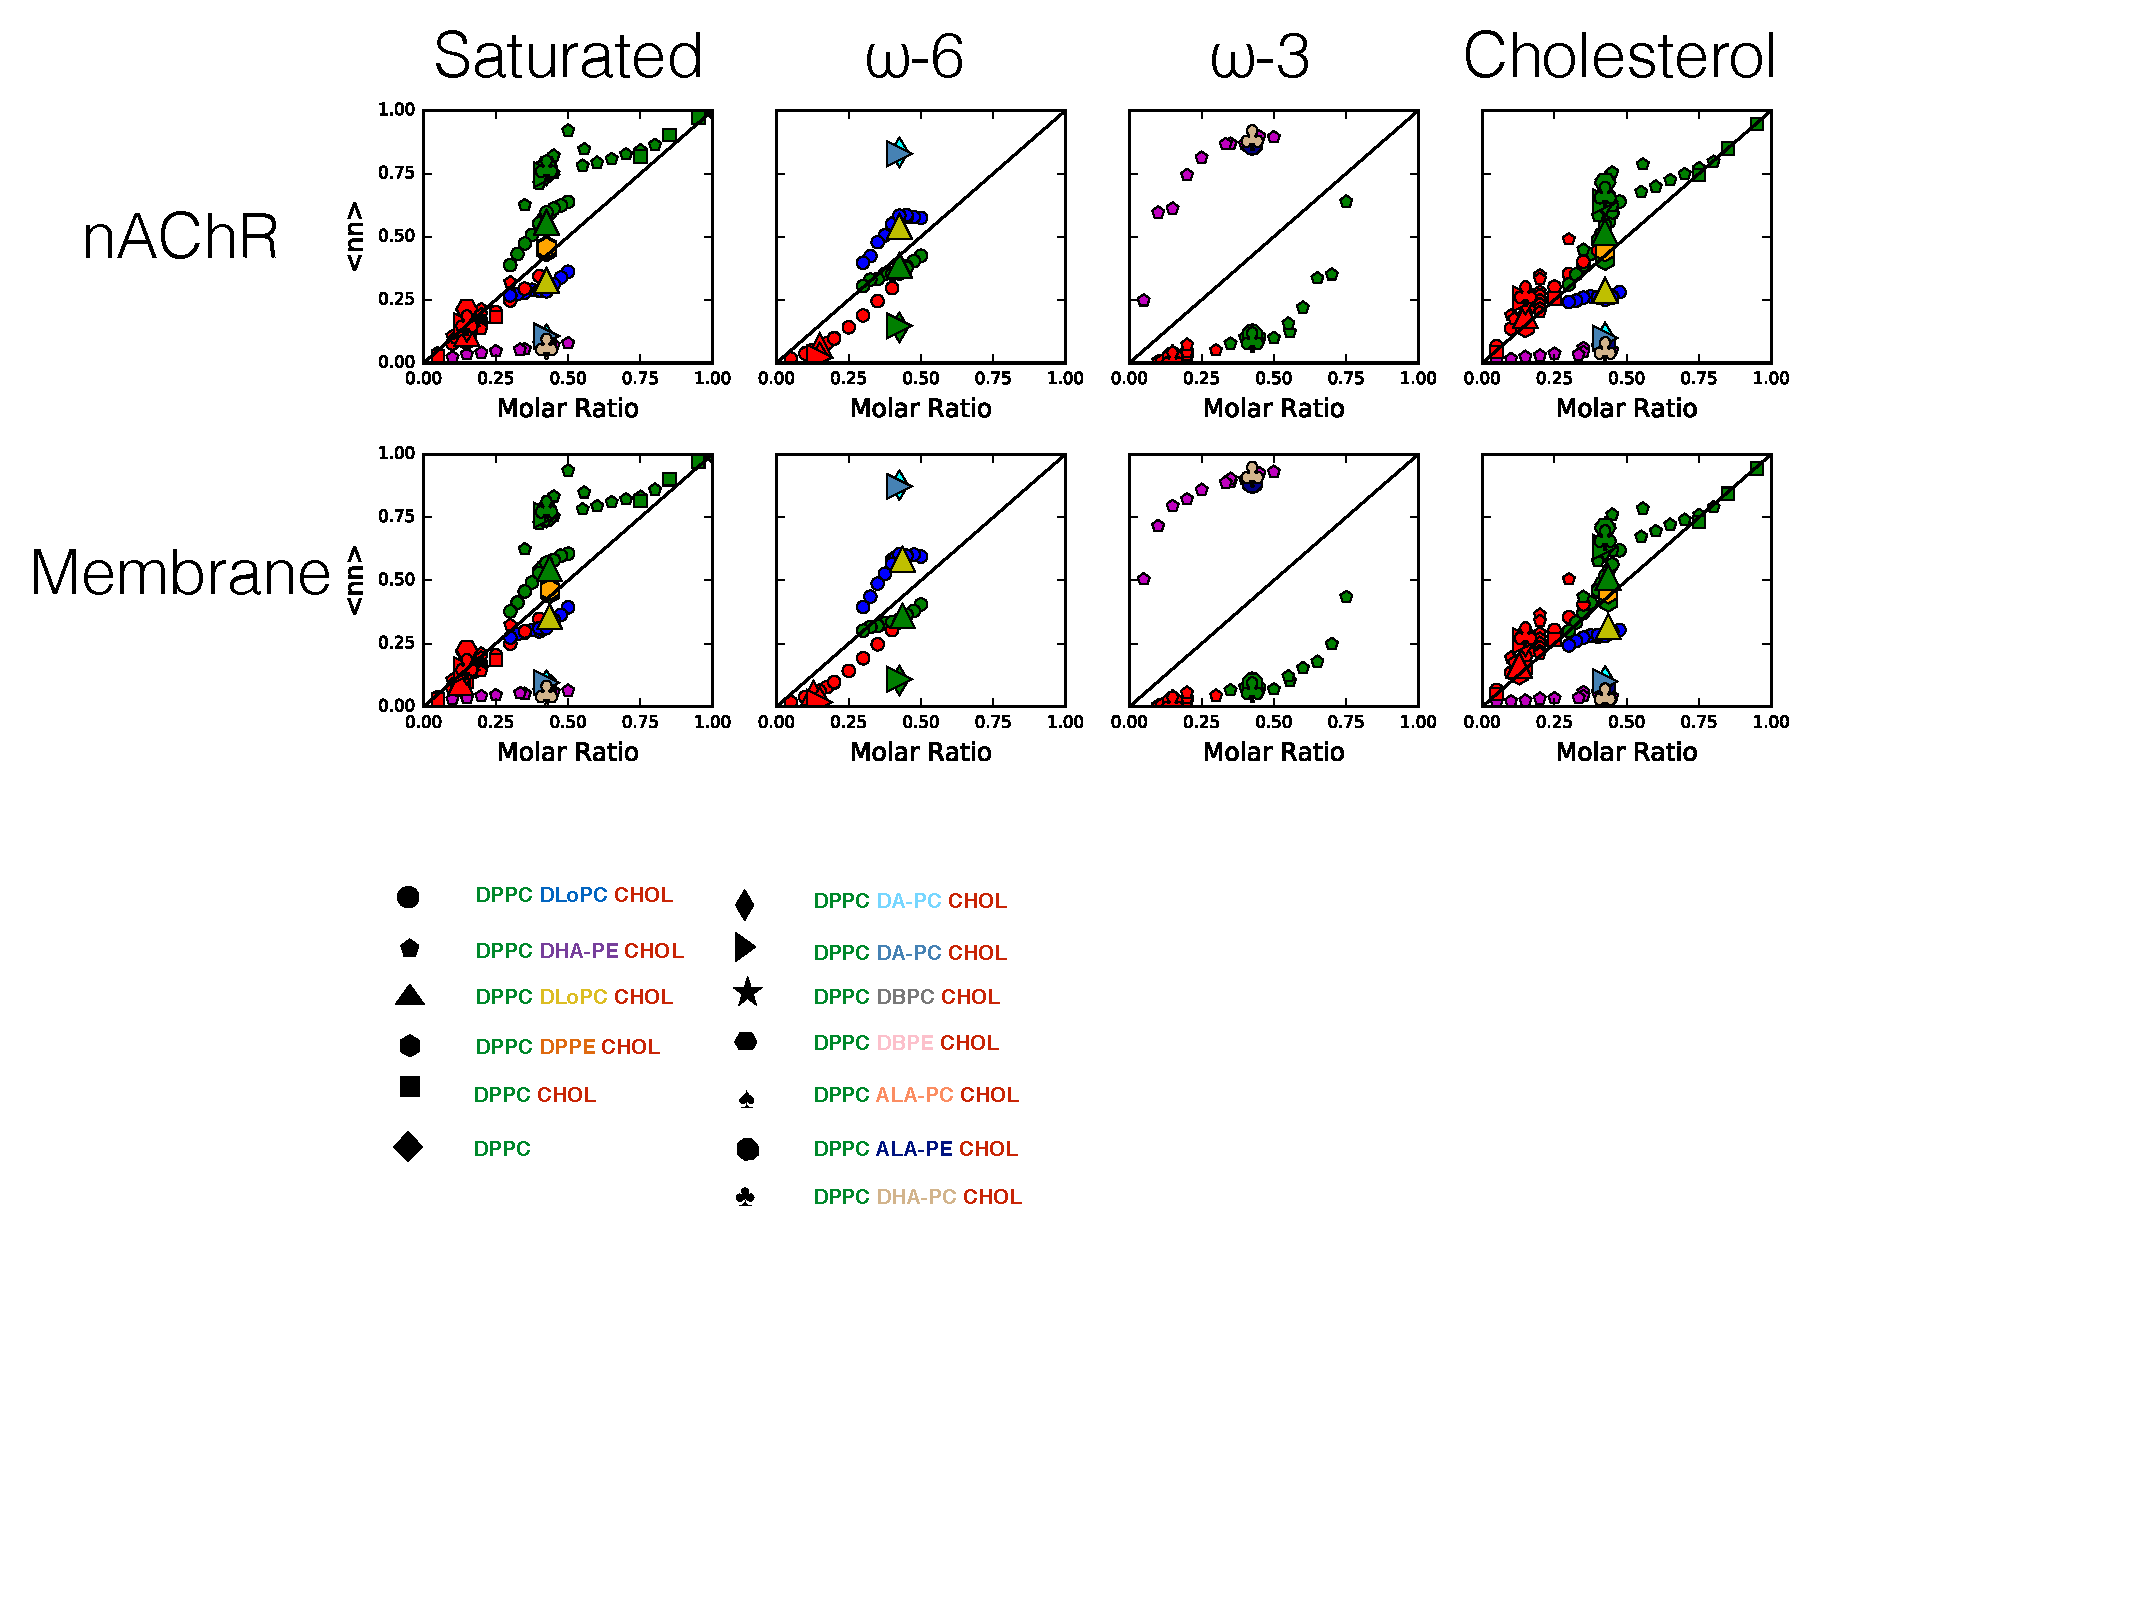
\includegraphics[width=\textwidth,scale=0.5]{NN.pdf}}
   \caption[Quantitative Analysis of Membrane Domain Formation]{\textbf{Quantitative Analysis of Membrane Domain Formation} Nearest neighbors are the six most likely lipids to surround a reference lipids. Expectation for a randomly mixed membrane is shown as the dashed line. As stated in the literature, saturated lipids and cholesterol mix forming liquid order domains. Short tailed $\omega$-6 lipids at low concentration appear to acutely mix with saturated lipids. $\omega$-3 unsaturated lipids do not mix with either unsaturated lipids or cholesterol. Images of systems at 42.5\% DPPC, 15\% cholesterol, and 42.5\% of secondary lipid can be seen for nAChR embedded, and nAChR free membranes in Figures \ref{fig:plips} and \ref{fig:mlips} respectively}\label{fig:nn}

\end{figure}
   \newpage

\begin{figure}[H]
   \centerline{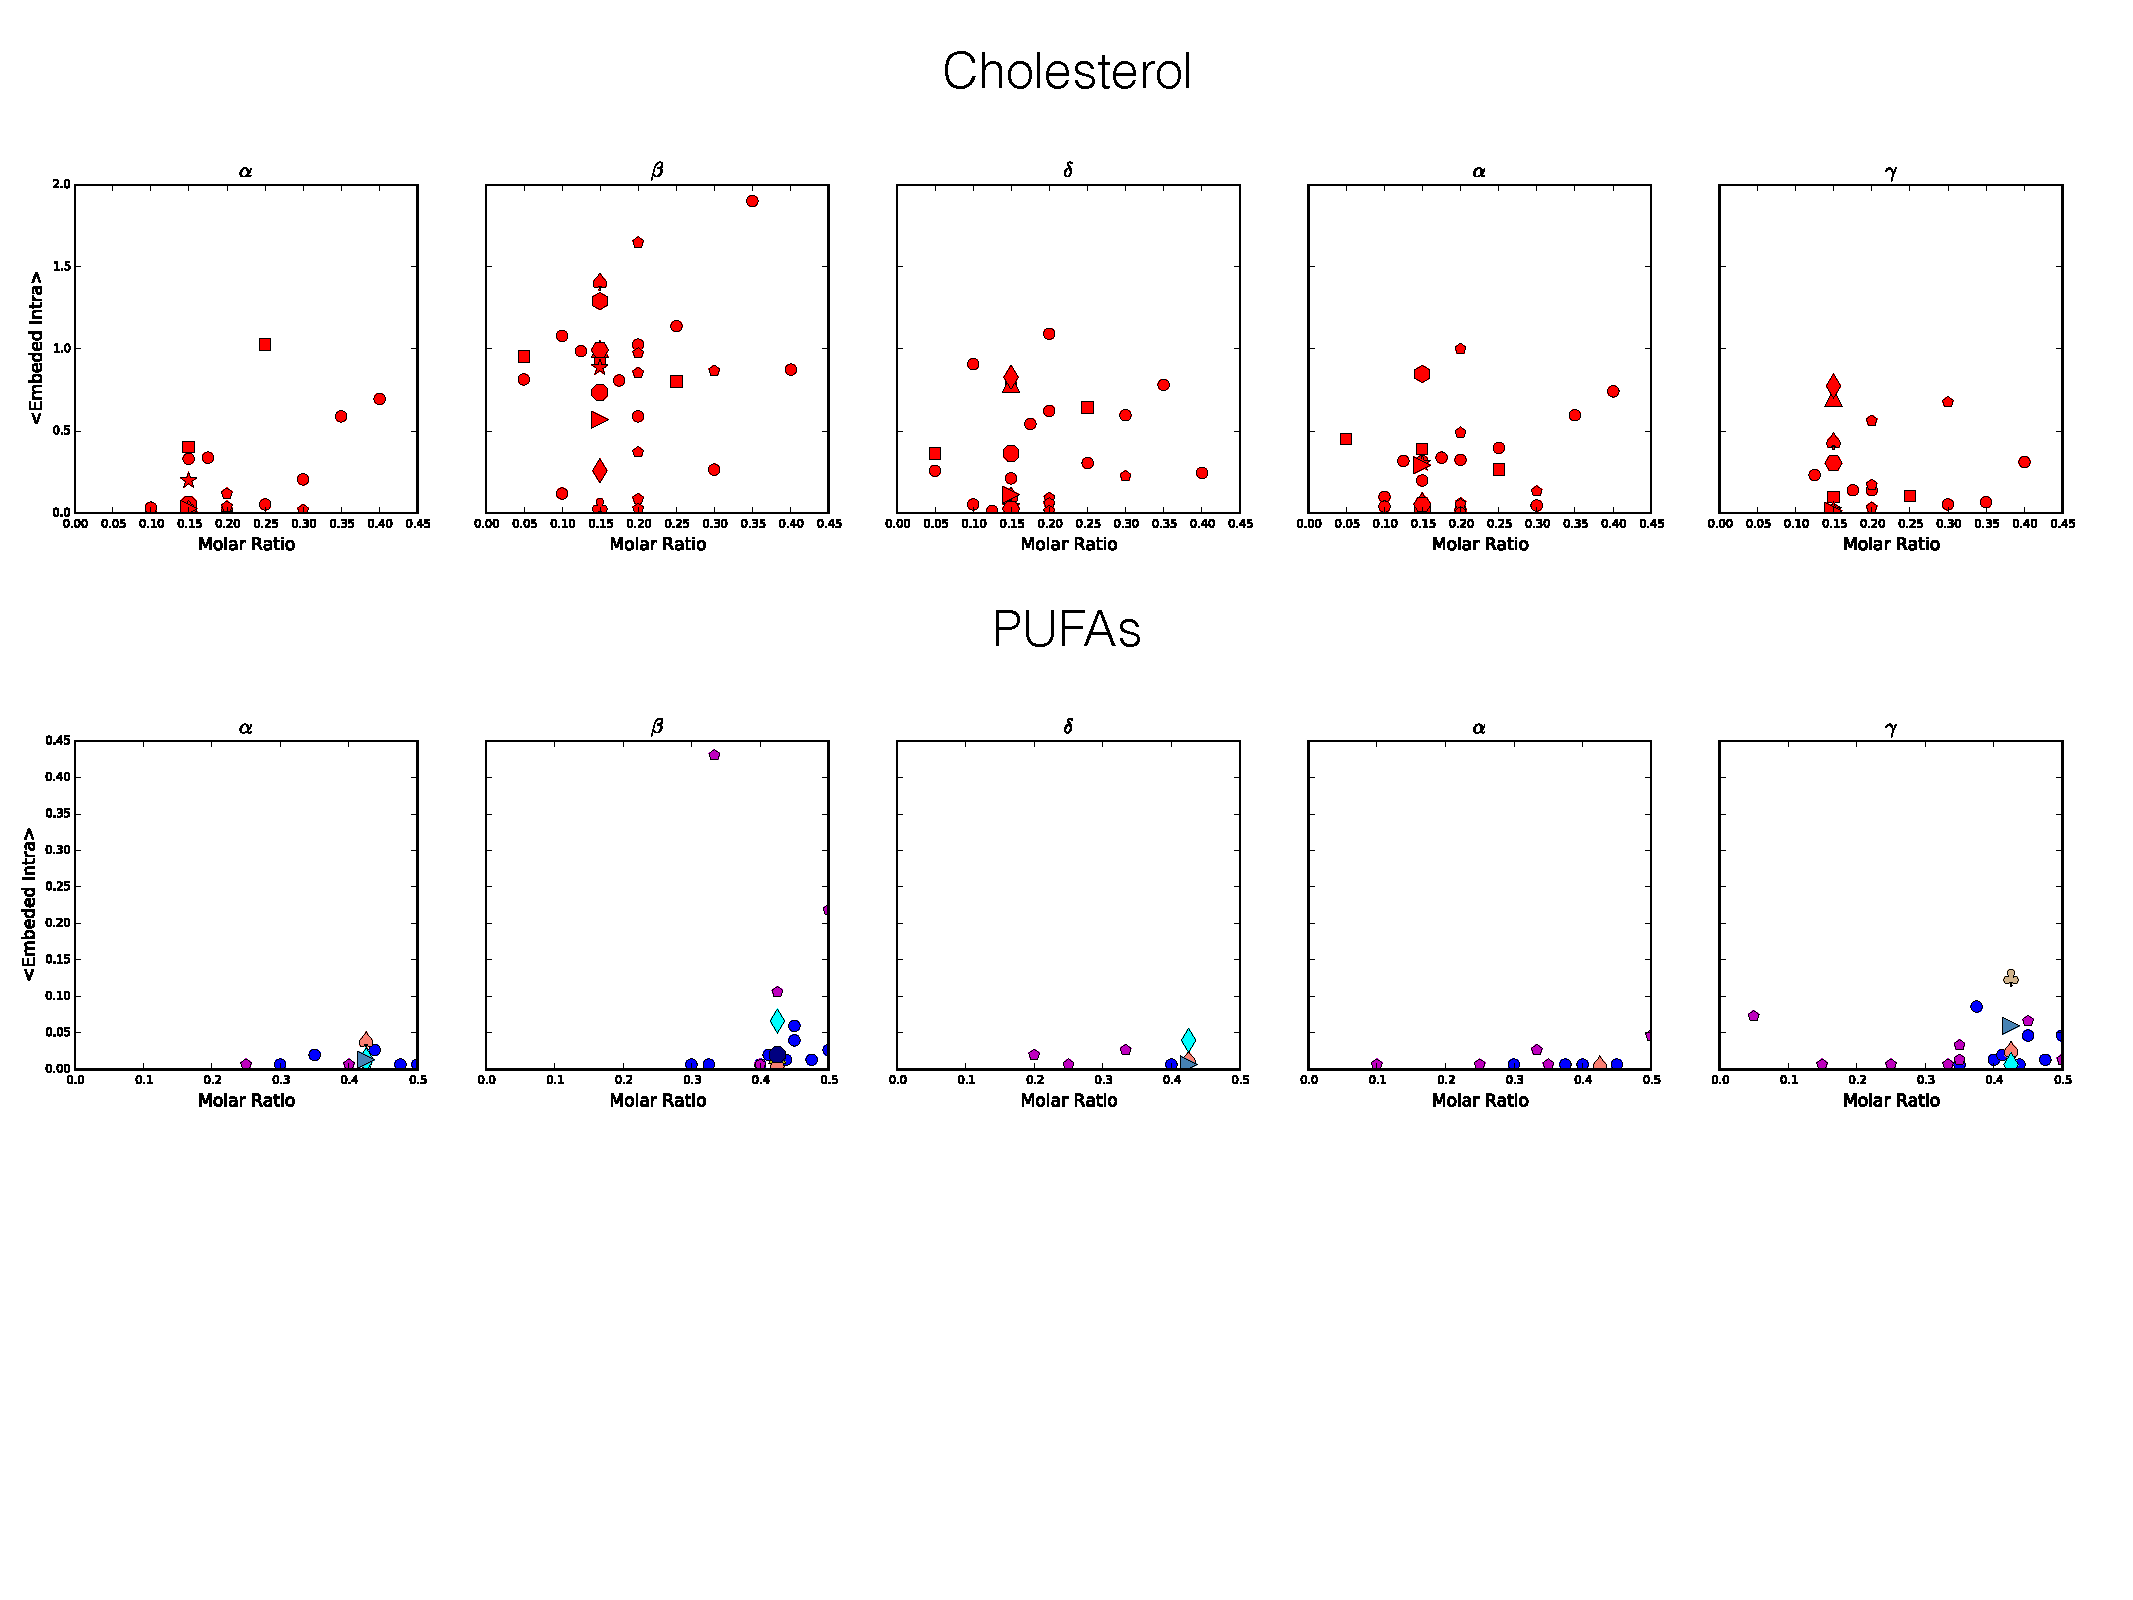
\includegraphics[width=\textwidth,scale=0.55]{Intra.pdf}}
   \centerline{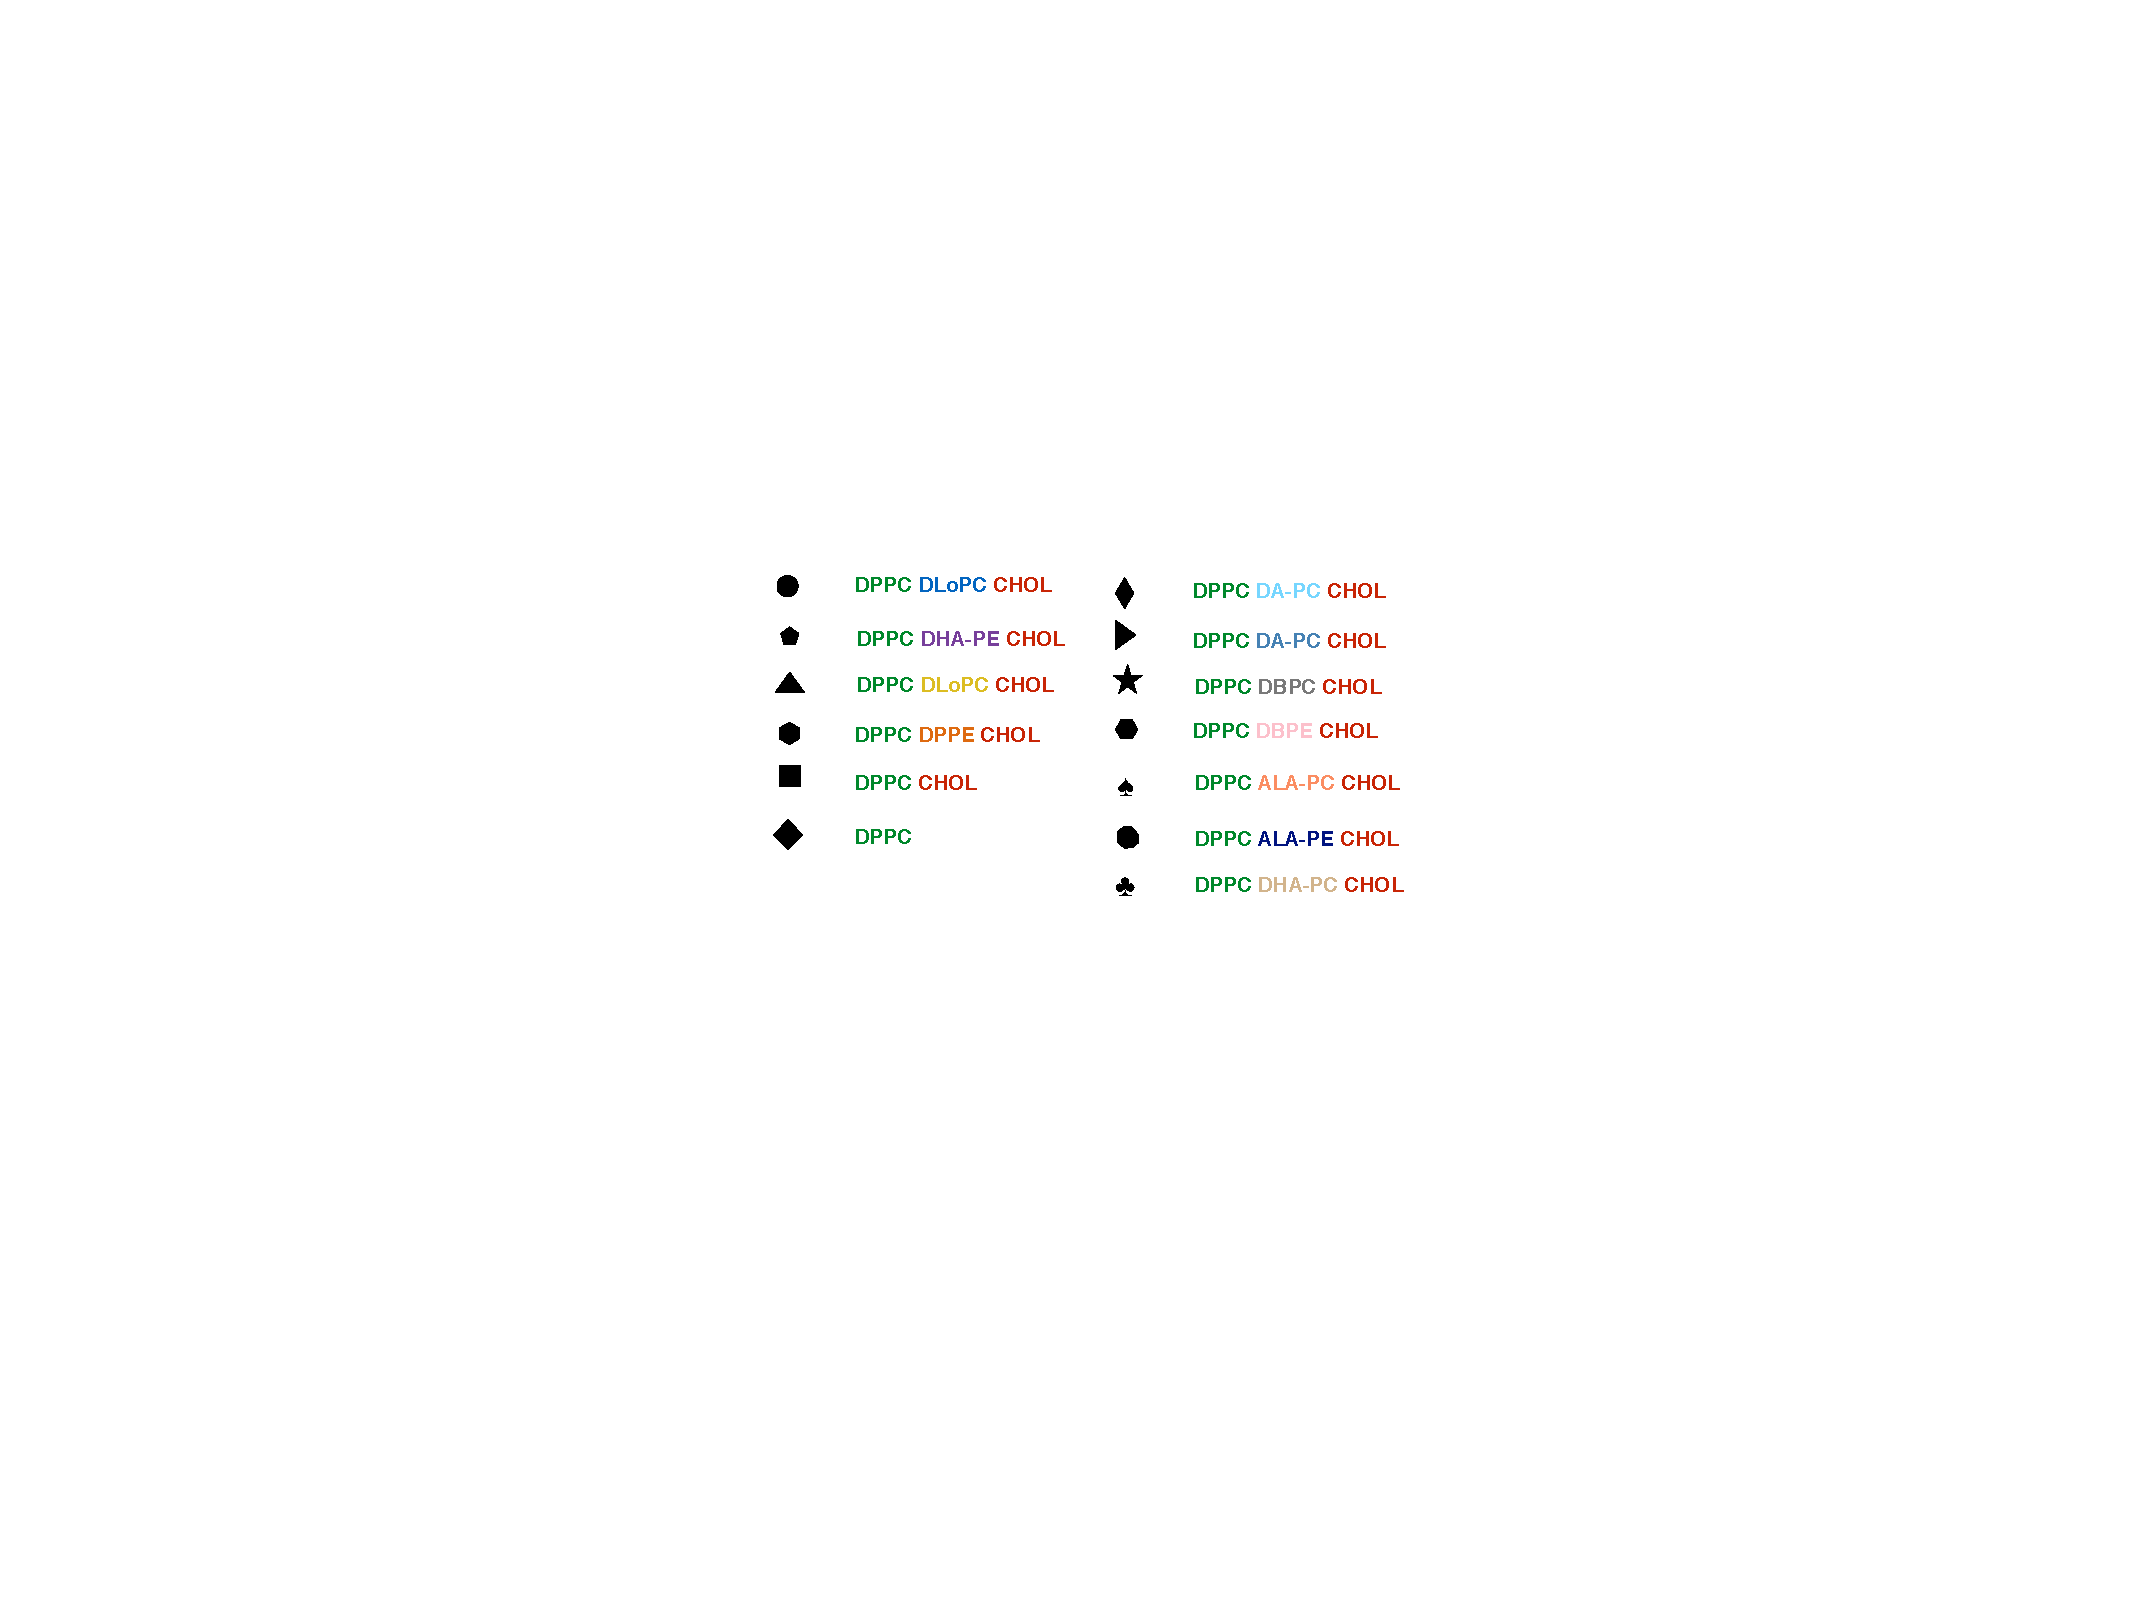
\includegraphics[scale=0.45]{Legend.pdf}}
   
   \caption[Quantitative Analysis of Embedded Lipids per Subunit]{\textbf{Quantitative Analysis of Embedded Lipids per Subunit} Cholesterol appears to prefer the $\beta$ subunit. While polyunsaturated lipids prefer the $\beta$ subunit, they do not appear to have the same affinity as cholesterol.}\label{fig:intra}
\end{figure}
   \newpage

\begin{figure}[H]
   \centerline{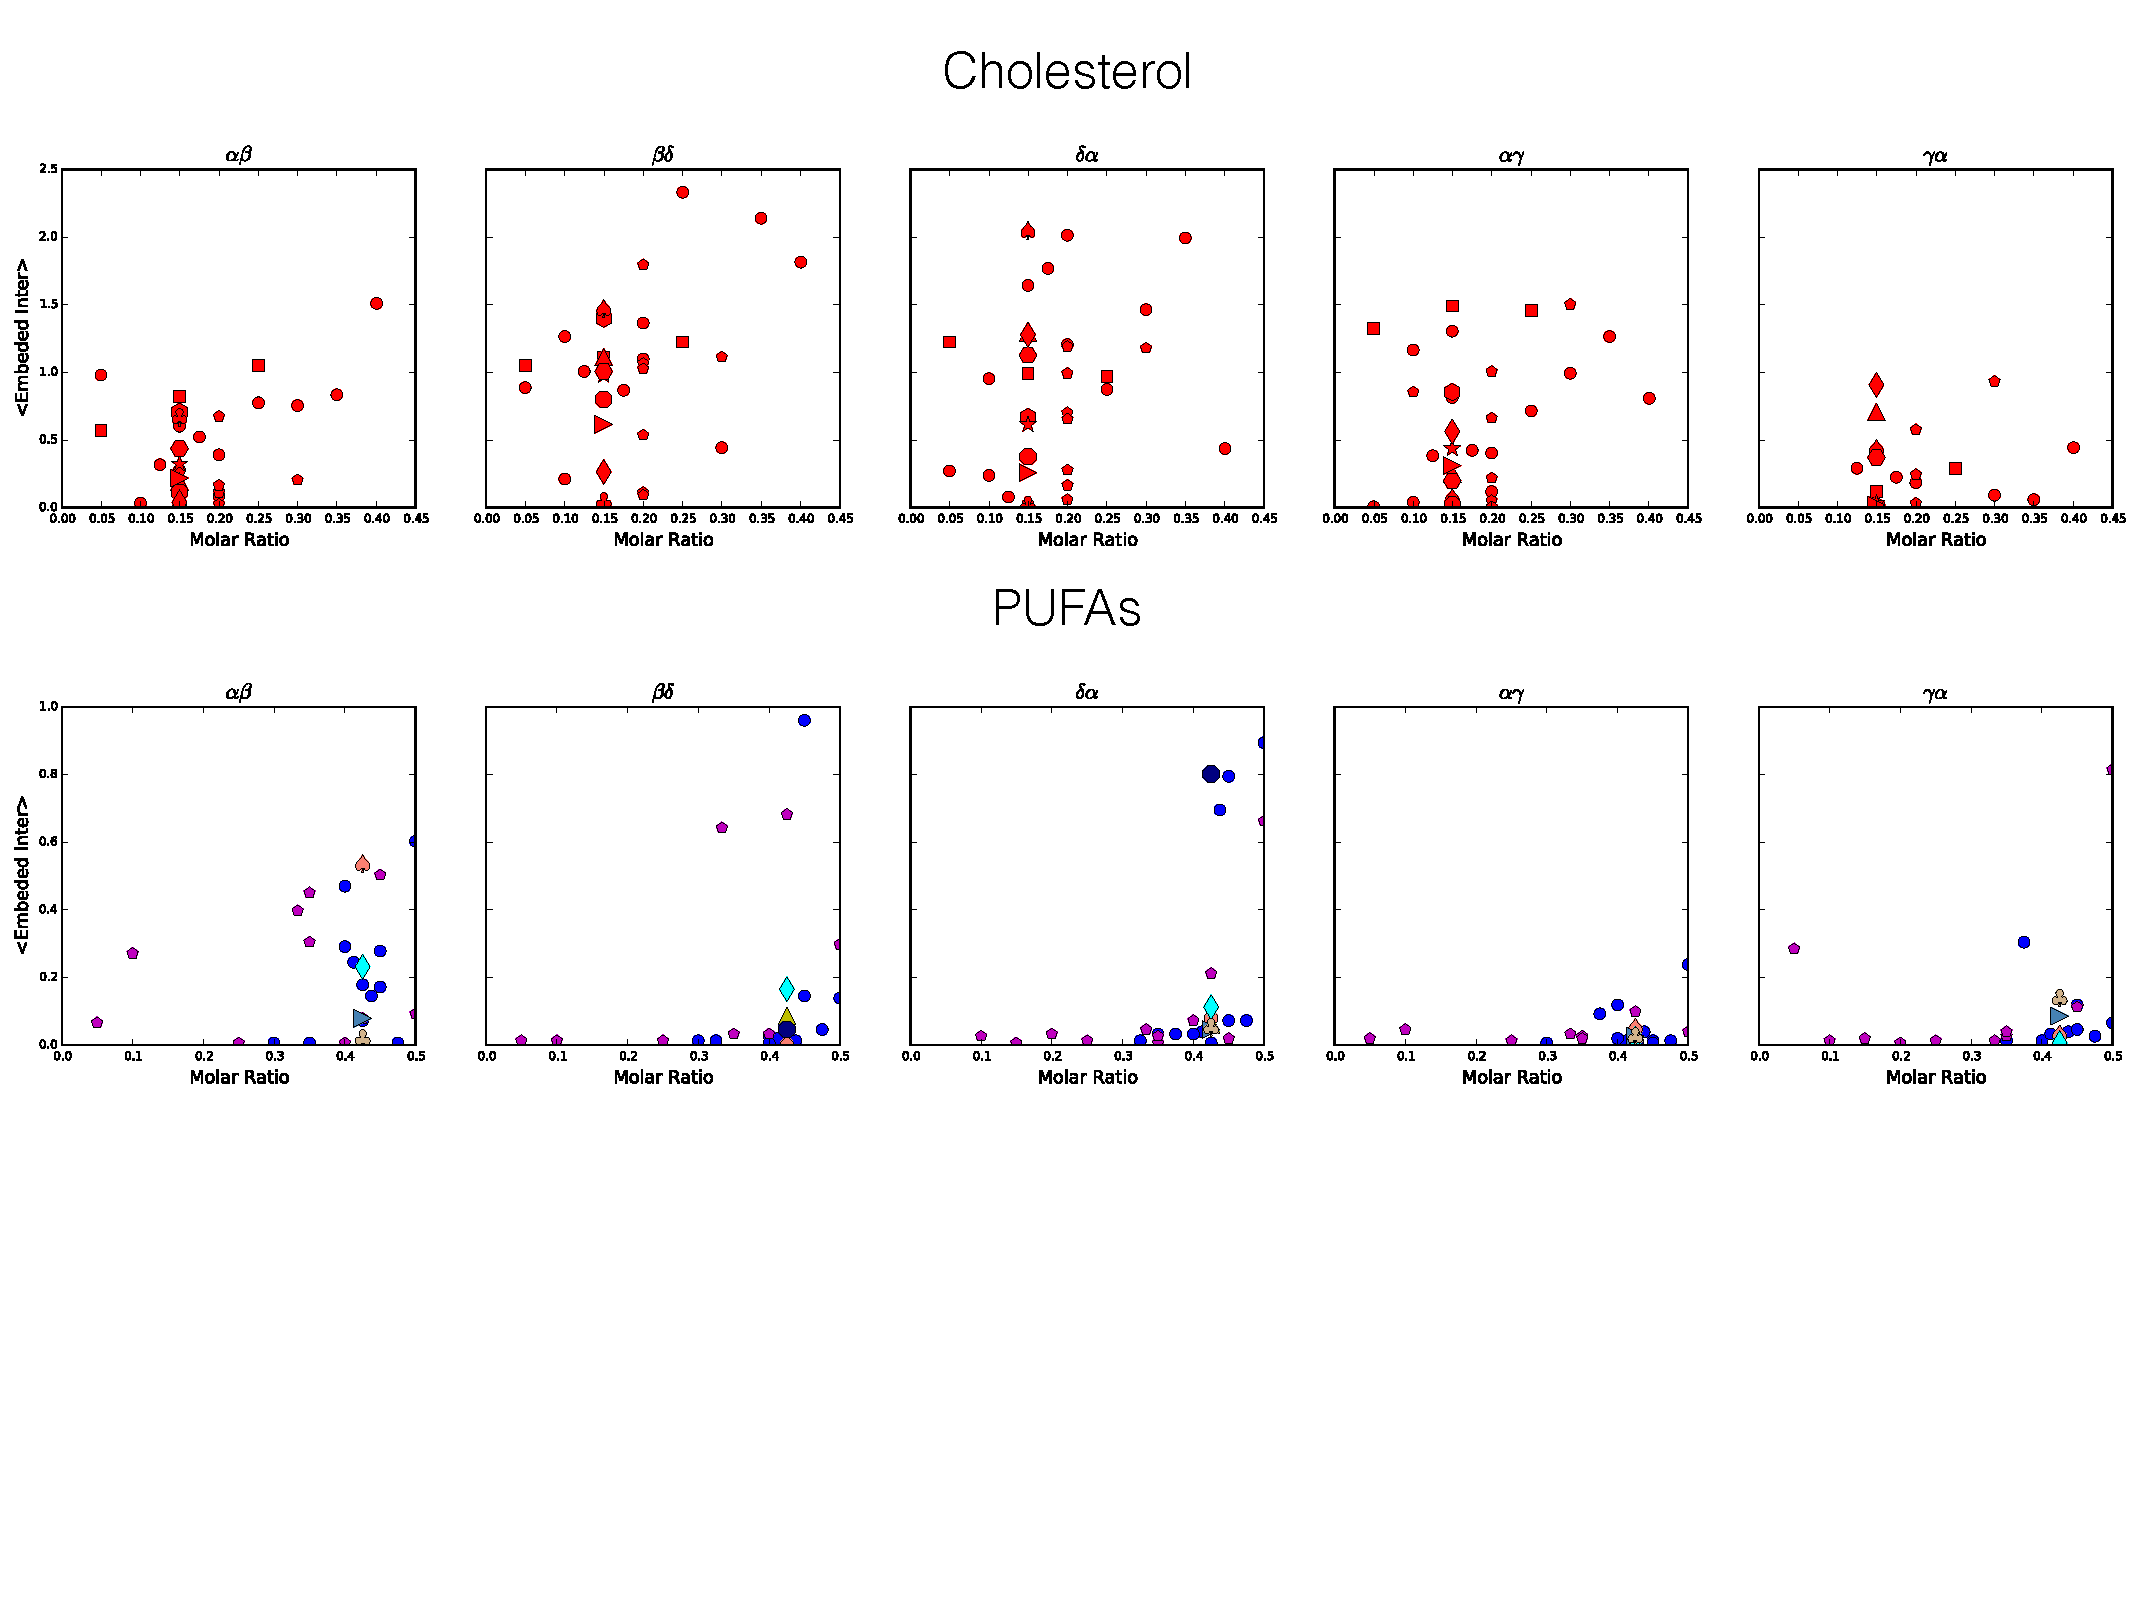
\includegraphics[width=\textwidth,scale=0.55]{Inter.pdf}}
   \centerline{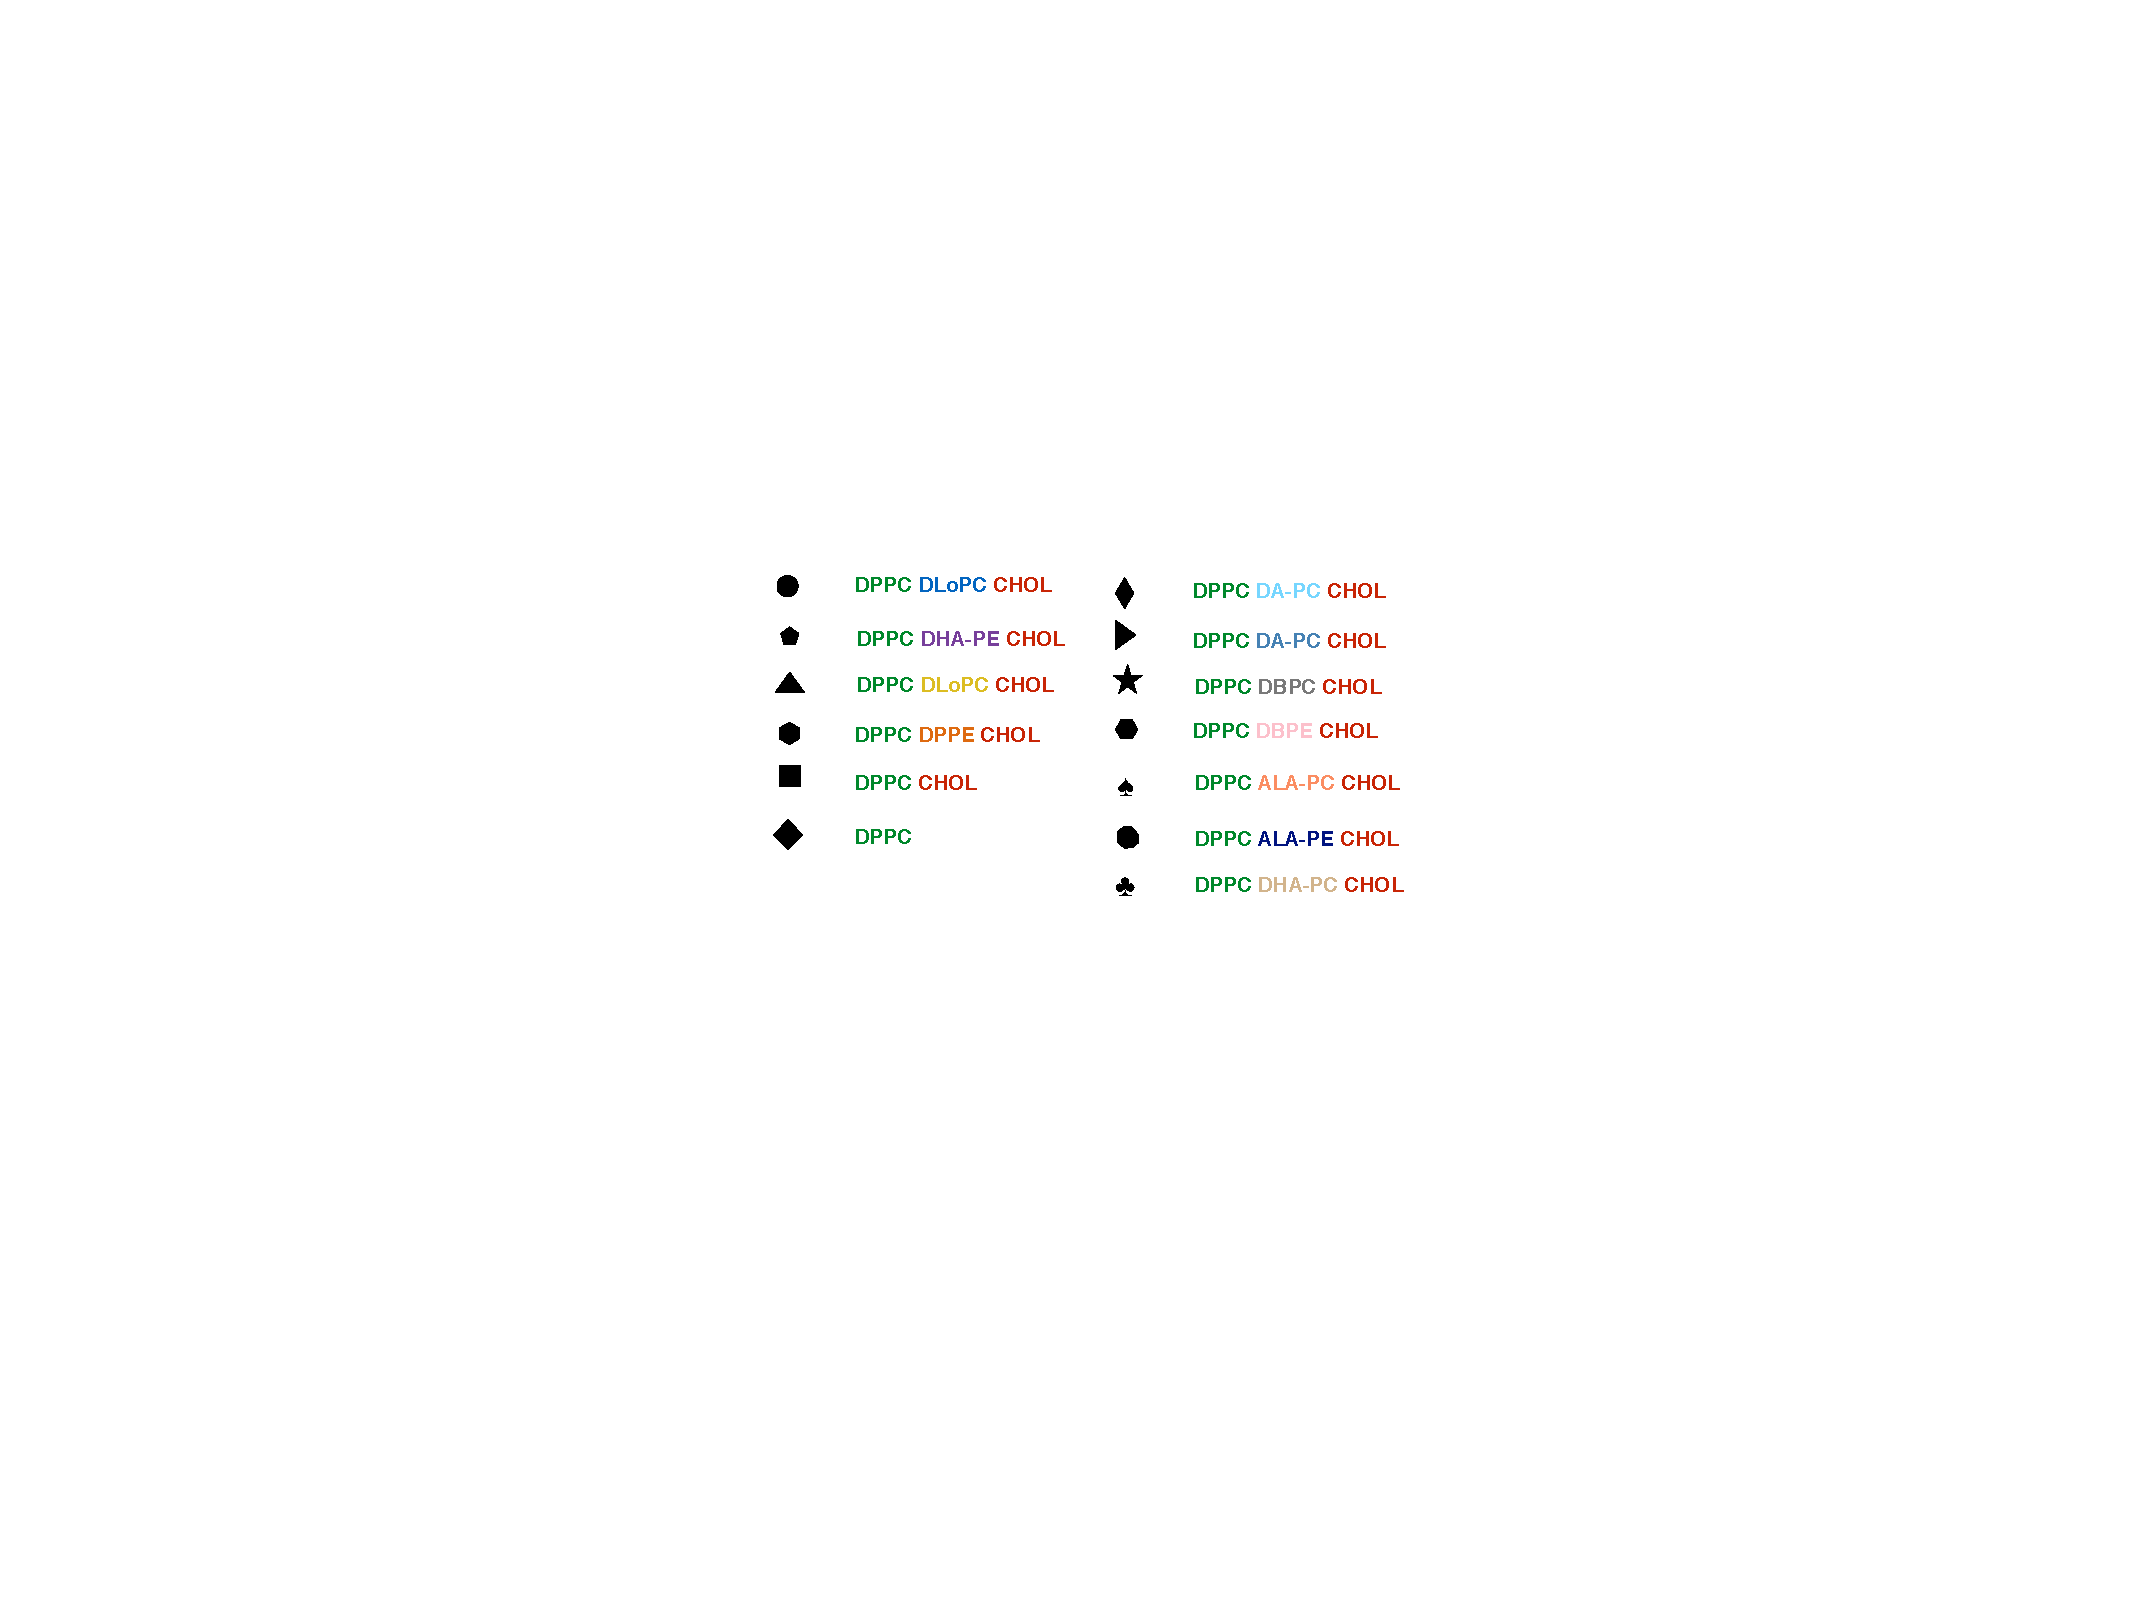
\includegraphics[scale=0.45]{Legend.pdf}}
   
   \caption[Quantitative Analysis of Embedded Lipids per Intersubunit]{\textbf{Quantitative Analysis of Embedded Lipids per Intersubunit} Cholesterol appears to have the weakest affinity with the intersubunits sharing faces with the $\alpha$ subunits. The polyunsaturated lipids with long tails seem to readily embed between the $\alpha\beta$, $\beta\delta$, and $\delta\alpha$ subunits.}\label{fig:inter}
\end{figure}
   \newpage

\section{Reference}
\linespread{1}
\printbibliography
\nocite{*}
\linespread{2}
\newpage


\end{document}